% Options for packages loaded elsewhere
% Options for packages loaded elsewhere
\PassOptionsToPackage{unicode}{hyperref}
\PassOptionsToPackage{hyphens}{url}
\PassOptionsToPackage{dvipsnames,svgnames,x11names}{xcolor}
%
\documentclass[
  ngerman,
  letterpaper,
  DIV=11]{scrreprt}
\usepackage{xcolor}
\usepackage{amsmath,amssymb}
\setcounter{secnumdepth}{5}
\usepackage{iftex}
\ifPDFTeX
  \usepackage[T1]{fontenc}
  \usepackage[utf8]{inputenc}
  \usepackage{textcomp} % provide euro and other symbols
\else % if luatex or xetex
  \usepackage{unicode-math} % this also loads fontspec
  \defaultfontfeatures{Scale=MatchLowercase}
  \defaultfontfeatures[\rmfamily]{Ligatures=TeX,Scale=1}
\fi
\usepackage{lmodern}
\ifPDFTeX\else
  % xetex/luatex font selection
\fi
% Use upquote if available, for straight quotes in verbatim environments
\IfFileExists{upquote.sty}{\usepackage{upquote}}{}
\IfFileExists{microtype.sty}{% use microtype if available
  \usepackage[]{microtype}
  \UseMicrotypeSet[protrusion]{basicmath} % disable protrusion for tt fonts
}{}
\makeatletter
\@ifundefined{KOMAClassName}{% if non-KOMA class
  \IfFileExists{parskip.sty}{%
    \usepackage{parskip}
  }{% else
    \setlength{\parindent}{0pt}
    \setlength{\parskip}{6pt plus 2pt minus 1pt}}
}{% if KOMA class
  \KOMAoptions{parskip=half}}
\makeatother
% Make \paragraph and \subparagraph free-standing
\makeatletter
\ifx\paragraph\undefined\else
  \let\oldparagraph\paragraph
  \renewcommand{\paragraph}{
    \@ifstar
      \xxxParagraphStar
      \xxxParagraphNoStar
  }
  \newcommand{\xxxParagraphStar}[1]{\oldparagraph*{#1}\mbox{}}
  \newcommand{\xxxParagraphNoStar}[1]{\oldparagraph{#1}\mbox{}}
\fi
\ifx\subparagraph\undefined\else
  \let\oldsubparagraph\subparagraph
  \renewcommand{\subparagraph}{
    \@ifstar
      \xxxSubParagraphStar
      \xxxSubParagraphNoStar
  }
  \newcommand{\xxxSubParagraphStar}[1]{\oldsubparagraph*{#1}\mbox{}}
  \newcommand{\xxxSubParagraphNoStar}[1]{\oldsubparagraph{#1}\mbox{}}
\fi
\makeatother

\usepackage{color}
\usepackage{fancyvrb}
\newcommand{\VerbBar}{|}
\newcommand{\VERB}{\Verb[commandchars=\\\{\}]}
\DefineVerbatimEnvironment{Highlighting}{Verbatim}{commandchars=\\\{\}}
% Add ',fontsize=\small' for more characters per line
\usepackage{framed}
\definecolor{shadecolor}{RGB}{241,243,245}
\newenvironment{Shaded}{\begin{snugshade}}{\end{snugshade}}
\newcommand{\AlertTok}[1]{\textcolor[rgb]{0.68,0.00,0.00}{#1}}
\newcommand{\AnnotationTok}[1]{\textcolor[rgb]{0.37,0.37,0.37}{#1}}
\newcommand{\AttributeTok}[1]{\textcolor[rgb]{0.40,0.45,0.13}{#1}}
\newcommand{\BaseNTok}[1]{\textcolor[rgb]{0.68,0.00,0.00}{#1}}
\newcommand{\BuiltInTok}[1]{\textcolor[rgb]{0.00,0.23,0.31}{#1}}
\newcommand{\CharTok}[1]{\textcolor[rgb]{0.13,0.47,0.30}{#1}}
\newcommand{\CommentTok}[1]{\textcolor[rgb]{0.37,0.37,0.37}{#1}}
\newcommand{\CommentVarTok}[1]{\textcolor[rgb]{0.37,0.37,0.37}{\textit{#1}}}
\newcommand{\ConstantTok}[1]{\textcolor[rgb]{0.56,0.35,0.01}{#1}}
\newcommand{\ControlFlowTok}[1]{\textcolor[rgb]{0.00,0.23,0.31}{\textbf{#1}}}
\newcommand{\DataTypeTok}[1]{\textcolor[rgb]{0.68,0.00,0.00}{#1}}
\newcommand{\DecValTok}[1]{\textcolor[rgb]{0.68,0.00,0.00}{#1}}
\newcommand{\DocumentationTok}[1]{\textcolor[rgb]{0.37,0.37,0.37}{\textit{#1}}}
\newcommand{\ErrorTok}[1]{\textcolor[rgb]{0.68,0.00,0.00}{#1}}
\newcommand{\ExtensionTok}[1]{\textcolor[rgb]{0.00,0.23,0.31}{#1}}
\newcommand{\FloatTok}[1]{\textcolor[rgb]{0.68,0.00,0.00}{#1}}
\newcommand{\FunctionTok}[1]{\textcolor[rgb]{0.28,0.35,0.67}{#1}}
\newcommand{\ImportTok}[1]{\textcolor[rgb]{0.00,0.46,0.62}{#1}}
\newcommand{\InformationTok}[1]{\textcolor[rgb]{0.37,0.37,0.37}{#1}}
\newcommand{\KeywordTok}[1]{\textcolor[rgb]{0.00,0.23,0.31}{\textbf{#1}}}
\newcommand{\NormalTok}[1]{\textcolor[rgb]{0.00,0.23,0.31}{#1}}
\newcommand{\OperatorTok}[1]{\textcolor[rgb]{0.37,0.37,0.37}{#1}}
\newcommand{\OtherTok}[1]{\textcolor[rgb]{0.00,0.23,0.31}{#1}}
\newcommand{\PreprocessorTok}[1]{\textcolor[rgb]{0.68,0.00,0.00}{#1}}
\newcommand{\RegionMarkerTok}[1]{\textcolor[rgb]{0.00,0.23,0.31}{#1}}
\newcommand{\SpecialCharTok}[1]{\textcolor[rgb]{0.37,0.37,0.37}{#1}}
\newcommand{\SpecialStringTok}[1]{\textcolor[rgb]{0.13,0.47,0.30}{#1}}
\newcommand{\StringTok}[1]{\textcolor[rgb]{0.13,0.47,0.30}{#1}}
\newcommand{\VariableTok}[1]{\textcolor[rgb]{0.07,0.07,0.07}{#1}}
\newcommand{\VerbatimStringTok}[1]{\textcolor[rgb]{0.13,0.47,0.30}{#1}}
\newcommand{\WarningTok}[1]{\textcolor[rgb]{0.37,0.37,0.37}{\textit{#1}}}

\usepackage{longtable,booktabs,array}
\usepackage{calc} % for calculating minipage widths
% Correct order of tables after \paragraph or \subparagraph
\usepackage{etoolbox}
\makeatletter
\patchcmd\longtable{\par}{\if@noskipsec\mbox{}\fi\par}{}{}
\makeatother
% Allow footnotes in longtable head/foot
\IfFileExists{footnotehyper.sty}{\usepackage{footnotehyper}}{\usepackage{footnote}}
\makesavenoteenv{longtable}
\usepackage{graphicx}
\makeatletter
\newsavebox\pandoc@box
\newcommand*\pandocbounded[1]{% scales image to fit in text height/width
  \sbox\pandoc@box{#1}%
  \Gscale@div\@tempa{\textheight}{\dimexpr\ht\pandoc@box+\dp\pandoc@box\relax}%
  \Gscale@div\@tempb{\linewidth}{\wd\pandoc@box}%
  \ifdim\@tempb\p@<\@tempa\p@\let\@tempa\@tempb\fi% select the smaller of both
  \ifdim\@tempa\p@<\p@\scalebox{\@tempa}{\usebox\pandoc@box}%
  \else\usebox{\pandoc@box}%
  \fi%
}
% Set default figure placement to htbp
\def\fps@figure{htbp}
\makeatother



\ifLuaTeX
\usepackage[bidi=basic]{babel}
\else
\usepackage[bidi=default]{babel}
\fi
% get rid of language-specific shorthands (see #6817):
\let\LanguageShortHands\languageshorthands
\def\languageshorthands#1{}
\ifLuaTeX
  \usepackage[german]{selnolig} % disable illegal ligatures
\fi


\setlength{\emergencystretch}{3em} % prevent overfull lines

\providecommand{\tightlist}{%
  \setlength{\itemsep}{0pt}\setlength{\parskip}{0pt}}



 


\KOMAoption{captions}{tableheading}
\makeatletter
\@ifpackageloaded{tcolorbox}{}{\usepackage[skins,breakable]{tcolorbox}}
\@ifpackageloaded{fontawesome5}{}{\usepackage{fontawesome5}}
\definecolor{quarto-callout-color}{HTML}{909090}
\definecolor{quarto-callout-note-color}{HTML}{0758E5}
\definecolor{quarto-callout-important-color}{HTML}{CC1914}
\definecolor{quarto-callout-warning-color}{HTML}{EB9113}
\definecolor{quarto-callout-tip-color}{HTML}{00A047}
\definecolor{quarto-callout-caution-color}{HTML}{FC5300}
\definecolor{quarto-callout-color-frame}{HTML}{acacac}
\definecolor{quarto-callout-note-color-frame}{HTML}{4582ec}
\definecolor{quarto-callout-important-color-frame}{HTML}{d9534f}
\definecolor{quarto-callout-warning-color-frame}{HTML}{f0ad4e}
\definecolor{quarto-callout-tip-color-frame}{HTML}{02b875}
\definecolor{quarto-callout-caution-color-frame}{HTML}{fd7e14}
\makeatother
\makeatletter
\@ifpackageloaded{bookmark}{}{\usepackage{bookmark}}
\makeatother
\makeatletter
\@ifpackageloaded{caption}{}{\usepackage{caption}}
\AtBeginDocument{%
\ifdefined\contentsname
  \renewcommand*\contentsname{Inhaltsverzeichnis}
\else
  \newcommand\contentsname{Inhaltsverzeichnis}
\fi
\ifdefined\listfigurename
  \renewcommand*\listfigurename{Abbildungsverzeichnis}
\else
  \newcommand\listfigurename{Abbildungsverzeichnis}
\fi
\ifdefined\listtablename
  \renewcommand*\listtablename{Tabellenverzeichnis}
\else
  \newcommand\listtablename{Tabellenverzeichnis}
\fi
\ifdefined\figurename
  \renewcommand*\figurename{Abbildung}
\else
  \newcommand\figurename{Abbildung}
\fi
\ifdefined\tablename
  \renewcommand*\tablename{Tabelle}
\else
  \newcommand\tablename{Tabelle}
\fi
}
\@ifpackageloaded{float}{}{\usepackage{float}}
\floatstyle{ruled}
\@ifundefined{c@chapter}{\newfloat{codelisting}{h}{lop}}{\newfloat{codelisting}{h}{lop}[chapter]}
\floatname{codelisting}{Listing}
\newcommand*\listoflistings{\listof{codelisting}{Listingverzeichnis}}
\makeatother
\makeatletter
\makeatother
\makeatletter
\@ifpackageloaded{caption}{}{\usepackage{caption}}
\@ifpackageloaded{subcaption}{}{\usepackage{subcaption}}
\makeatother
\usepackage{bookmark}
\IfFileExists{xurl.sty}{\usepackage{xurl}}{} % add URL line breaks if available
\urlstyle{same}
\hypersetup{
  pdftitle={Unterlagen für das obligatorische Fach Informatik},
  pdfauthor={Jacques Mock Schindler},
  pdflang={de},
  colorlinks=true,
  linkcolor={blue},
  filecolor={Maroon},
  citecolor={Blue},
  urlcolor={Blue},
  pdfcreator={LaTeX via pandoc}}


\title{Unterlagen für das obligatorische Fach Informatik}
\author{Jacques Mock Schindler}
\date{02.10.2025}
\begin{document}
\maketitle

\renewcommand*\contentsname{Inhaltsverzeichnis}
{
\hypersetup{linkcolor=}
\setcounter{tocdepth}{2}
\tableofcontents
}

\bookmarksetup{startatroot}

\chapter*{Willkommen}\label{willkommen}
\addcontentsline{toc}{chapter}{Willkommen}

\markboth{Willkommen}{Willkommen}

Hier finden Sie die Informationen für den Informatikunterricht.

\section*{Programm}\label{programm}
\addcontentsline{toc}{section}{Programm}

\markright{Programm}

\begin{longtable}[]{@{}ll@{}}
\toprule\noalign{}
Datum & Thema \\
\midrule\noalign{}
\endhead
\bottomrule\noalign{}
\endlastfoot
18.08.2025 & Was ist Informatik \\
25.08.2025 & Vorbereiten der Arbeitsumgebung \\
01.09.2025 & Problemlösung in der Informatik \\
08.09.2025 & Variablen als Wegweiser zu Objekten \\
15.09.2025 & Schlaufen \\
22.09.2025 & Bedingungen \\
20.10.2025 & Anwendungsübung \\
27.10.2025 & Individuelle Prüfungsvorbereitung \\
03.11.2025 & Test \\
10.11.2025 & Datenstrukturen \\
17.11.2025 & Datenstrukturen \\
24.11.2025 & Algorithmen \\
01.12.2025 & Algorithmen \\
08.12.2025 & Wiederholung ohne Schleife (Rekursion) \\
15.12.2025 & Anwendungsübungen \\
05.01.2026 & Individuelle Prüfungsvorbereitung \\
12.01.2026 & Test \\
\end{longtable}

Das Programm widerspiegelt den aktuellen Stand der Planung. Es ist im
Verlauf des Semesters mit Änderungen zu rechnen.

\section*{Materielle Voraussetzungen}\label{materielle-voraussetzungen}
\addcontentsline{toc}{section}{Materielle Voraussetzungen}

\markright{Materielle Voraussetzungen}

Für den Informatikunterricht ist ein Laptop erforderlich (mit einem iPad
können Sie die im Unterricht gestellten Aufgaben nicht lösen). Für Ihren
Laptop brachen Sie zur Installation der erforderlichen Software
Administratorenrechte.\\
Ausserdem müssen Sie sicherstellen, dass Ihr Akku zu Beginn des
Unterrichts einen Ladestand aufweist, der eine Doppelstunde durchhält.

\section*{Beurteilung}\label{beurteilung}
\addcontentsline{toc}{section}{Beurteilung}

\markright{Beurteilung}

Pro Semester sind zwei schriftliche Prüfungen vorgesehen. Ausserdem wird
die mündliche Beteiligung benotet. Als mündliche Beteiligung gilt
insbesondere auch das Stellen von Fragen.\\
Die Zeugnisnote berechnet sich als gewichteter Durchschnitt aus den
beiden schriftlichen Prüfungen und der Note für die mündliche
Beteiligung. Die Durchschnittsnote der beiden schriftlichen Prüfungen
wird mit 90\%, die Note für die mündliche Beteiligung mit 10\%
gewichtet.

Falls jemand eine persönliche Besprechung wünscht, kann sich hier für
eine Sprechstunde anmelden (Rent a Mock).

\part{Anleitungen}

\chapter{Speicherorganisation}\label{speicherorganisation}

Informationen sind in Computern in Dateien gespeichert. Die
gespeicherten Informationen können dabei ganz unterschiedlicher Art, wie
zum Beispiel Texte, Bilder oder Videos, sein.\\
Als Modell, wie man sich Dateien vorstellen kann, hat sich das Bild von
Dossiers in Ordnern etabliert. Die einzelnen Dossiers sind die Dateien
und die Ordner sind die Strukturen, in denen die Dateien abgelegt sind.
Diese Konstruktion kann über mehrere Ebenen hinaus verschachtelt werde
(Ordner in Gestellen, die wiederum in einzelnen Räumen stehen, etc.).

\section{Dateinamen und Pfade}\label{dateinamen-und-pfade}

Damit Dateien identifiziert und gefunden werden können, müssen sie einen
Namen haben. Grundsätzlich gibt es keine Einschränkungen, wie Dateien
benannt werden. Die meisten Dateinamen bestehen allerdings aus zwei
Teilen: dem eigentlichen Dateinamen und der Dateinamenserweiterung.

Der eigentliche Dateiname wird idealerweise so festgelegt, dass er einen
Rückschluss auf den Inhalt der Datei zulässt.\\
Die Dateinamenserweiterung ist ein Zusatz, der Auskunft über den
Dateityp gibt. Sie steht hinter einem Punkt hinter dem eigentlichen
Dateinamen. Auf Windows Rechnern wird die Dateinamenserweiterung im
Dateimanager in der Standardeinstellung nicht angezeigt. Um dies zu
ändern, muss in den Einstellungen des Dateimanagers die Option
``Dateinamenerweiterungen anzeigen'' aktiviert werden (Ansicht
\textgreater{} Anzeigen \textgreater{} Dateinamenserweiterung).

Damit Dateien besser ausgetauscht werden können, empfiehlt es sich, für
die Namen lediglich Buchstaben, Zahlen und Unterstriche (sog.
\href{https://de.wikipedia.org/wiki/American_Standard_Code_for_Information_Interchange}{ASCII}-Zeichen)
zu verwenden.

Damit man Dateien finden kann, muss man wissen, wo sie abgelegt worden
sind. Übertragen auf das Modell von Dossiers in Ordnern bedeutet das, zu
wissen, welches Dossier in welchem Ordner in welchem Gestell in welchem
Raum abgelegt ist. Wie in einem realen Archiv, geht man dabei vom Raum
zum Gestell, zum Ordner und schliesslich zum Dossier. In der Informatik
wird dieser Weg als Pfad bezeichnet. Auf einem Windows-Rechner beginnt
dieser Pfad mit dem sogenannten Laufwerksbuchstaben, gefolgt von einem
Doppelpunkt und einem Backslash (\texttt{\textbackslash{}}). Aus
historischen Gründen ist der Laufwerksbuchstabe auf Windows-Rechnern
Standardmässig der Buchstabe \texttt{C}.

Ein Beispiel für einen Pfad könnte so aussehen:

\begin{Shaded}
\begin{Highlighting}[numbers=left,,]
\ExtensionTok{C:\textbackslash{}Users\textbackslash{}fritz\textbackslash{}Documents\textbackslash{}text.docx}
\end{Highlighting}
\end{Shaded}

In diesem Beispiel ist \texttt{C:} der Laufwerksbuchstabe,
\texttt{Users} der Ordner, \texttt{fritz} der Unterordner,
\texttt{Documents} der Unterordner von \texttt{fritz} und
\texttt{text.docx} die Datei, die im Ordner \texttt{Documents} abgelegt
ist. \texttt{Users} ist ein von Windows standardmässig angelegter
Ordner, in dem die persönlichen Daten der Benutzer abgelegt werden. Der
Ordner \texttt{fritz} ist der persönliche Ordner des Benutzers
\texttt{fritz}. Der Ordner \texttt{Documents} wird ebenfalls
standardmässig von Windows im Ordner jedes Benutzers angelegt. Dem
Benutzer \texttt{fritz} steht es frei, diesen Ordner zu verwenden und
darin Dateien oder Underordner anzulegen.\\
Der Dateiname \texttt{text.docx} verweist mit seiner
Dateinamenserweiterung \texttt{.docx} auf eine Datei, die mit dem
Programm Microsoft Word erstellt worden ist.

\section{Dateien in der Cloud}\label{dateien-in-der-cloud}

Dateien können nicht nur lokal auf dem Computer gespeichert werden.
Damit von überall und jederzeit auf Dateien zugegriffen werden kann,
werden Dateien in der \emph{Cloud} gespeichert. Dabei handelt es sich um
Server in Rechenzentren, die über das Internet erreichbar sind.
Beispiele für solche Cloud-Dienst sind OneDrive von Microsoft oder
Google Drive.\\
Ablageorte auf OneDrive werden in Windows direkt in der
Verzeichnisstruktur des Betriebssystems angezeigt, solche von Google
erhalten auf Windows einen eigenen Laufwerksbuchstaben
(\texttt{G:\textbackslash{}}).

Damit auf die Dateien in der Cloud zugegriffen werden kann, ist eine
Internetverbindung erforderlich.

\section{Dateistruktur für die
Schule}\label{dateistruktur-fuxfcr-die-schule}

Für den schulischen Bedarf erscheint es sinnvoll eine Dateistruktur nach
Fächern anzulegen. Im Ordner \texttt{Documents} wird dazu für jedes Fach
ein eigener Unterordner angelegt. Innerhalb der jeweiligen Fachordner
kann eine weitere Struktur nach Semester oder nach Thema sinnvoll sein.
Ein Beispiel für die Ordnerstruktur eines Erstklässlers an der KBW kann
so aussehen:

\begin{Shaded}
\begin{Highlighting}[numbers=left,,]
\NormalTok{Documents\textbackslash{}}
\NormalTok{         ├──Schule\textbackslash{}}
\NormalTok{         |       ├──Deutsch}
\NormalTok{         |       ├──Franz}
\NormalTok{         |       ├──Mathe}
\NormalTok{         |       ├──WR}
\NormalTok{         |       └──...}
\NormalTok{         ├──Privat\textbackslash{}}
\NormalTok{         |       ├──Rechnungen}
\NormalTok{         |       └──...}
\end{Highlighting}
\end{Shaded}

\chapter{Arbeitsumgebung (Arbeiten mit Jupyter
Notebooks)}\label{arbeitsumgebung-arbeiten-mit-jupyter-notebooks}

\section{Ausgangslage}\label{ausgangslage}

In der Informatik geht es darum, wie Informationsverarbeitung mit Hilfe
von Computern automatisiert werden kann.\\
Die Automatisierung der Informationsverarbeitung erfordert die
Verwendung von Programmiersprachen. Im Informatikunterricht wird in
erster Linie mit der Programmiersprache Python gearbeitet.\\
Im folgenden findet sich eine Anleitung für die Installation der für den
Unterricht erforderlichen Programme.

\section{Installation von Python}\label{installation-von-python}

Dieser Abschnitt führt Sie Schritt für Schritt durch die Installation
von Python auf einem Windows-Rechner.

\begin{tcolorbox}[enhanced jigsaw, leftrule=.75mm, toprule=.15mm, title=\textcolor{quarto-callout-warning-color}{\faExclamationTriangle}\hspace{0.5em}{Microsoft Store Falle}, bottomrule=.15mm, breakable, rightrule=.15mm, colback=white, left=2mm, colbacktitle=quarto-callout-warning-color!10!white, coltitle=black, arc=.35mm, bottomtitle=1mm, opacitybacktitle=0.6, toptitle=1mm, colframe=quarto-callout-warning-color-frame, opacityback=0, titlerule=0mm]

Achten Sie beim Herunterladen von Python darauf, dass Sie sich auf der
offiziellen Seite von Python (https://www.python.org) und \textbf{nicht}
im Microsoft Store befinden. Wenn Sie versehentlich die Python Version
aus dem Microsoft Store installiert haben, kann das bei der Arbeit an
den Schulprojekten zu Problemen führen.

Deinstallieren Sie die Microsoft Version von Python und installieren Sie
die Version von der offiziellen Website.

\end{tcolorbox}

\begin{enumerate}
\def\labelenumi{\arabic{enumi}.}
\item
  Laden Sie die neueste Version von Python von der offiziellen Website
  herunter: python.org.
\item
  Führen Sie das heruntergeladene Installationsprogramm durch
  Doppelklick auf die Datei aus. Stellen Sie sicher, dass Sie die Option
  ``Add Python to PATH'' aktivieren, bevor Sie auf ``Install Now''
  klicken.

  \begin{tcolorbox}[enhanced jigsaw, leftrule=.75mm, toprule=.15mm, title=\textcolor{quarto-callout-tip-color}{\faLightbulb}\hspace{0.5em}{Die `PATH'-Umgebungsvariable}, bottomrule=.15mm, breakable, rightrule=.15mm, colback=white, left=2mm, colbacktitle=quarto-callout-tip-color!10!white, coltitle=black, arc=.35mm, bottomtitle=1mm, opacitybacktitle=0.6, toptitle=1mm, colframe=quarto-callout-tip-color-frame, opacityback=0, titlerule=0mm]

  Stellen Sie sich die PATH-Variable wie ein Adressbuch für die
  Kommandozeile (Terminal) vor. Wenn Sie einen Befehl wie
  \texttt{python} eingeben, schaut der Computer in diesem Adressbuch
  nach, wo das entsprechende Programm zu finden ist.

  Indem Sie das Häkchen bei ``Add Python to PATH'' setzen, fügen Sie die
  Adresse des Python-Interpreters zu diesem Adressbuch hinzu. Ohne
  diesen Eintrag weiss der Computer nicht, wo er suchen soll, und
  meldet, dass er den Befehl nicht kennt.

  \end{tcolorbox}
\item
  Überprüfen Sie die Installation, indem Sie die Eingabeaufforderung
  öffnen (Terminal \(\rightarrow\) Windows-Taste + R, dann \texttt{cmd}
  eingeben) und den Befehl \texttt{python\ -\/-version} eingeben. Dies
  sollte die installierte Python-Version anzeigen.
\end{enumerate}

\section{Hello World}\label{hello-world}

Es hat sich eingebürgert, dass das erste Programm, das ausgeführt wird,
ein Programm ist, das den Text ``Hello World'' auf dem Bildschirm
ausgibt. Um dieser Tradition zu folgen, führen Sie die folgenden
Schritte aus:

\begin{enumerate}
\def\labelenumi{\arabic{enumi}.}
\item
  Öffnen Sie ein Terminal (Windows-Taste + R, dann \texttt{cmd}
  eingeben).

  \begin{tcolorbox}[enhanced jigsaw, leftrule=.75mm, toprule=.15mm, title=\textcolor{quarto-callout-tip-color}{\faLightbulb}\hspace{0.5em}{Das Terminal}, bottomrule=.15mm, breakable, rightrule=.15mm, colback=white, left=2mm, colbacktitle=quarto-callout-tip-color!10!white, coltitle=black, arc=.35mm, bottomtitle=1mm, opacitybacktitle=0.6, toptitle=1mm, colframe=quarto-callout-tip-color-frame, opacityback=0, titlerule=0mm]

  Unter dem Begriff ``Terminal'' versteht man ein Programm, das eine
  textbasierte Benutzeroberfläche bereitstellt, um mit dem
  Betriebssystem zu interagieren. In einem Terminal können Sie Befehle
  eingeben und erhalten die Ausgaben direkt im Fenster.

  \end{tcolorbox}
\item
  Geben Sie den Befehl \texttt{python} ein, um die Python-Shell zu
  starten. Die Python Shell sollte ungefähr so, wie das folgende Bild
  aussehen.

  \begin{figure}[H]

  {\centering \pandocbounded{\includegraphics[keepaspectratio]{files/lektionen_hs25/250702_systemeinrichtung/python_shell.png}}

  }

  \caption{Python Shell}

  \end{figure}%
\item
  Geben Sie den folgenden Befehl ein und drücken Sie anschliessend die
  Eingabetaste:

\begin{Shaded}
\begin{Highlighting}[numbers=left,,]
\BuiltInTok{print}\NormalTok{(}\StringTok{"Hello World"}\NormalTok{)}
\end{Highlighting}
\end{Shaded}

  Das Resultat sollte wie das folgende Bild aussehen.

  \begin{figure}[H]

  {\centering \pandocbounded{\includegraphics[keepaspectratio]{files/lektionen_hs25/250702_systemeinrichtung/hello_world.png}}

  }

  \caption{Python Shell}

  \end{figure}%
\end{enumerate}

Gratuliere - Sie haben Ihr erstes Python-Programm erfolgreich
ausgeführt!

\section{Arbeitsumgebung}\label{arbeitsumgebung}

Im Unterricht wird nicht direkt in der Python-Shell gearbeitet, sondern
mit sogenannten Jupyter Notebooks. Jupyter Notebooks ermöglichen es, in
der gleichen Datei sowohl Code (Programm Teile) als auch formatierten
Text (in Markdown) zu verarbeiten. Eine Jupyter Notebook Datei hat die
Endung \texttt{.ipynb}. Vom Jupyter Notebook unterschieden werden muss
die Arbeitsoberfläche in welcher die Jupyter Notebooks bearbeitet
werden. Diese Oberfläche nennt sich JupyterLab und läuft in einem
Webbrowser.

\begin{tcolorbox}[enhanced jigsaw, leftrule=.75mm, toprule=.15mm, title=\textcolor{quarto-callout-tip-color}{\faLightbulb}\hspace{0.5em}{Das Jupyter Ökosystem}, bottomrule=.15mm, breakable, rightrule=.15mm, colback=white, left=2mm, colbacktitle=quarto-callout-tip-color!10!white, coltitle=black, arc=.35mm, bottomtitle=1mm, opacitybacktitle=0.6, toptitle=1mm, colframe=quarto-callout-tip-color-frame, opacityback=0, titlerule=0mm]

Die im Unterricht verwendeten Jupyter Notebooks sind Teil eines ganzen
Jupyter Ökosystems. Der Name Jupyter setzt sich aus den drei
Programmiersprachen \textbf{Ju}lia, \textbf{Pyt}hon und \textbf{R}
zusammen, die in diesem Ökosystem eine zentrale Rolle spielen. Zum
Jupyter Ökosystem gehören auch zahlreiche Erweiterungen und Tools, die
die Arbeit mit Notebooks und Daten erleichtern.

Der Unterricht beschränkt sich auf die Verwendung von Jupyter Notebooks
mit der Programmiersprache Python sowie den Einsatz von JupyterLab als
Arbeitsumgebung.

\end{tcolorbox}

Damit dies alles funktioniert, braucht es ein paar weitere
Vorbereitungsarbeiten.

\begin{enumerate}
\def\labelenumi{\arabic{enumi}.}
\item
  Erstellen Sie im Ordner ``Informatik'' einen Unterordner mit dem
  Heutigen Datum als Namen. Formatieren Sie das Datum nach dem Schema
  ``YYMMDD'', für den 1. August 2025 wäre das zum Beispiel ``250801''.
\item
  Öffnen Sie den soeben erstellten Ordner.
\item
  Geben Sie die Tastenfolge \texttt{Ctrl\ +\ L} ein, um die Adresszeile
  des Dateimanagers zu aktivieren.
\item
  Überschreiben Sie den Inhalt der Adresszeile mit dem Text \texttt{cmd}
  und drücken Sie die Eingabetaste. Dadurch wird ein Terminal geöffnet,
  das direkt im aktuellen Ordner arbeitet.
\item
  Geben Sie im neu geöffneten Terminal den folgenden Befehl ein und
  drücken Sie die Eingabetaste:

\begin{Shaded}
\begin{Highlighting}[numbers=left,,]
\ExtensionTok{python} \AttributeTok{{-}m}\NormalTok{ venv .venv}
\end{Highlighting}
\end{Shaded}

  Dadurch wird eine sogenannte Python Virtual Environment erstellt (venv
  wegen \textbf{V}irtual \textbf{Env}ironment). Dieses Python Virtual
  Environment dient dazu, die eigenen Programmierprojekte unabhängig
  voneinander gestalten zu können.
\item
  Aktivieren Sie das Python Virtual Environment mit dem folgenden
  Befehl:

\begin{Shaded}
\begin{Highlighting}[numbers=left,,]
 \ExtensionTok{.venv\textbackslash{}Scripts\textbackslash{}activate}
\end{Highlighting}
\end{Shaded}

  Ihr Terminal sieht nach dem Erstellen und Aktivieren der Python
  Virtual Environment ungefähr so aus:

  \begin{figure}[H]

  {\centering \pandocbounded{\includegraphics[keepaspectratio]{files/lektionen_hs25/250702_systemeinrichtung/venv.png}}

  }

  \caption{Aktivierte Python Virtual Environment}

  \end{figure}%

  Das Wort in der Klammer am Anfang der Zeile zeigt den Namen der
  aktiven Python Virtual Environment an. Im vorliegenden Fall ist das
  .venv.
\item
  \phantomsection\label{sec-install-packages}{In der nun aktivierten
  Python Virtual Environment installieren Sie die benötigten Pakete mit
  dem folgenden Befehl}:

\begin{Shaded}
\begin{Highlighting}[numbers=left,,]
\ExtensionTok{pip}\NormalTok{ install jupyter}
\end{Highlighting}
\end{Shaded}

  Das dauert eine Weile.

  Während der Installation werden die benötigten Pakete (Ergänzungen zur
  bestehenden Python Installation) heruntergeladen und in der Python
  Virtual Environment gespeichert. Das Terminal sieht dabei ungefähr so
  aus:

  \begin{figure}[H]

  {\centering \pandocbounded{\includegraphics[keepaspectratio]{files/lektionen_hs25/250702_systemeinrichtung/installation.png}}

  }

  \caption{Terminal während der Jupyter Installation}

  \end{figure}%

  Alle in einer Python Virtual Environment installierten Pakete sind
  innerhalb dieser Umgebung dauerhaft verfügbar und müssen daher für das
  gleiche Projekt kein zweites Mal installiert werden.
\item
  Starten Sie den Jupyter Server mit dem folgenden Befehl:

\begin{Shaded}
\begin{Highlighting}[numbers=left,,]
 \ExtensionTok{jupyter{-}lab}
\end{Highlighting}
\end{Shaded}

  Dies startet den Jupyter Notebook Server und öffnet automatisch ein
  Browserfenster mit der Jupyter Notebook Oberfläche.

  \begin{figure}[H]

  {\centering \pandocbounded{\includegraphics[keepaspectratio]{files/lektionen_hs25/250702_systemeinrichtung/server.png}}

  }

  \caption{Startseite Jupyter Lab}

  \end{figure}%
\item
  Klicken Sie auf den Button ``Python 3 (ipykernel)'' unter dem Titel
  Notebook.

  Damit starten Sie ein neues Jupyter Notebook. Der Cursor blinkt in
  einer leeren Zelle. Bei dieser Zelle handelt es sich um eine
  sogenannte Code-Zelle. In einer Code-Zelle können Sie Python Code
  eingeben und ausführen.\\
  Überprüfen Sie das, indem Sie in der Zelle den Befehl
  \texttt{print("Hello\ World")} eingeben und anschliessend die
  Tastenfolge \texttt{Shift\ +\ Enter} drücken (alternativ können Sie
  auch auf den Button ``Run'' in der Werkzeugleiste klicken).

  Das Resultat sollte wie das folgende Bild aussehen.

  \begin{figure}[H]

  {\centering \pandocbounded{\includegraphics[keepaspectratio]{files/lektionen_hs25/250702_systemeinrichtung/hello_world_ipynb.png}}

  }

  \caption{Hello World in einem Jupyter Notebook}

  \end{figure}%

  In einem Jupyter Notebook können Sie nicht nur Python Code ausführen,
  sondern auch Text (formatiert in Markdown) darstellen.\\
  Für die Darstellung von Text müssen Sie die Zelle als Text-Zelle
  markieren. Dazu klicken Sie auf den Button ``Code'' in der
  Werkzeugleiste und wählen im Dropdown-Menü die Option ``Markdown''
  aus.

  \begin{figure}[H]

  {\centering \pandocbounded{\includegraphics[keepaspectratio]{files/lektionen_hs25/250702_systemeinrichtung/cell_switch.png}}

  }

  \caption{Umstellen der Zelle auf Markdown}

  \end{figure}%

  Probieren Sie das aus. Schreiben Sie einen Titel und einen kurzen Text
  in die Zelle unterhalb der Code-Zelle mit
  \texttt{pringt("Hello\ World")}. Damit der Text in der Zelle
  formatiert angezeigt wird, müssen Sie die Zelle mit der Tastenfolge
  \texttt{Shift\ +\ Enter} ausführen (analog zum Ausführen von
  Code-Zellen).

  Eine Zelle ist entweder eine Code-Zelle oder eine Text-Zelle. Für den
  Wechsel zwischen Code- und Text-Darstellung müssen Sie je eine neue
  Zelle anlegen. Das geht mit der Tastenfolge \texttt{Esc\ +\ B} (für
  ``Below'') oder \texttt{Esc\ +\ A} (für ``Above'') während Sie sich in
  einer Zelle befinden. Alternativ können Sie auch die Buttons ``Insert
  Cell Below'' oder ``Insert Cell Above'' aus den Werkzeugen der Zelle
  verwenden.
\item
  Das Jupyter Notebook ist eine Datei mit der Endung \texttt{.ipynb}.
  Neu erstellte Jupyter Notebooks erhalten den Namen ``Untitled.ipynb''.
  Um diesen Namen zu ändern, klicken Sie mit der rechten Maustatste auf
  den Titel ``Untitled'' in der oberen linken Ecke des Jupyter Notebooks
  und wählen Sie die Option ``Rename'' aus dem Kontextmenü.
  Anschliessend können Sie den Namen des Jupyter Notebooks eingeben.
\end{enumerate}

\section{Öffnen bestehender Jupyter
Notebooks}\label{uxf6ffnen-bestehender-jupyter-notebooks}

Häufiger als das Erstellen eines neuen Jupyter Notebooks ist das Öffnen
eines bereits bestehenden Jupyter Notebooks. Hier wird das entsprechende
Vorgehen beschrieben.

\begin{enumerate}
\def\labelenumi{\arabic{enumi}.}
\item
  Navigieren Sie in den Ordner in dem sich das Jupyter Notebook
  befindet.
\item
  Stellen Sie sicher, dass der Ordner über eine Python Virtual
  Environment mit installierten Jupyter Paketen verfügt.

  Öffnen Sie dazu im ausgewählten Ordner das Terminal
  (\texttt{ctrl\ +\ L} anschliessend \texttt{cmd} und Eingabetaste).
  Dann starten Sie die Python Virtual Environment und geben den Befehl
  \texttt{pip\ list} ein. Dieser Listet alle in der Python Virtual
  Environment installierten Pakete auf. Falls die Jupyter Pakete nicht
  aufgelistet werden, müssen Sie diese wie
  \hyperref[sec-install-packages]{oben} beschrieben installieren.
\item
  Starten Sie den Jupyter Server mit dem Befehl \texttt{jupyter-lab}.
\item
  Öffnen Sie das Dateiverzeichnis. Dazu müssen Sie auf dem linken Rand
  das Ordner-Symbol anklicken.
\item
  Wählen Sie das Jupyter Notebook aus, das Sie öffnen möchten. Mit einem
  Doppelklick auf das Jupyter Notebook wird dieses geöffnet.

  Wenn Sie das Dateiverzeichnis wieder schliessen möchten, klicken Sie
  auf das Ordner-Symbol auf der linken Seite erneut.
\end{enumerate}

Diese Schritte funktionieren auch, wenn Sie ein Jupyter Notebook öffnen
möchten, das Sie von jemand anderem erhalten haben. Sie müssen dieses
dazu lediglich in den Ordner kopieren, in dem sich die Python Virtual
Environment mit den installierten Jupyter Paketen befindet.

\section{Häufige Fehlermeldungen}\label{huxe4ufige-fehlermeldungen}

\begin{longtable}[]{@{}
  >{\raggedright\arraybackslash}p{(\linewidth - 4\tabcolsep) * \real{0.3333}}
  >{\raggedright\arraybackslash}p{(\linewidth - 4\tabcolsep) * \real{0.3333}}
  >{\raggedright\arraybackslash}p{(\linewidth - 4\tabcolsep) * \real{0.3333}}@{}}
\toprule\noalign{}
\begin{minipage}[b]{\linewidth}\raggedright
Problem / Fehlermeldung (Was Sie sehen)
\end{minipage} & \begin{minipage}[b]{\linewidth}\raggedright
Mögliche Ursache (Warum es passiert)
\end{minipage} & \begin{minipage}[b]{\linewidth}\raggedright
Lösung (Was Sie tun können)
\end{minipage} \\
\midrule\noalign{}
\endhead
\bottomrule\noalign{}
\endlastfoot
Der Befehl \texttt{python} ist entweder falsch geschrieben oder konnte
nicht gefunden werden. & Python wurde bei der Installation nicht zur
PATH-Variable hinzugefügt. Der Computer weiss nicht, wo er
\texttt{python.exe} finden soll. &
\begin{minipage}[t]{\linewidth}\raggedright
\begin{enumerate}
\tightlist
\item
  Deinstallieren Sie Python über die Systemsteuerung.
\item
  Installieren Sie Python erneut.
\item
  Achten Sie diesmal unbedingt darauf, das Häkchen bei "Add Python to
  PATH" zu setzen.
\end{enumerate}
\end{minipage} \\
Der Befehl \texttt{jupyter-lab} ist entweder falsch geschrieben oder
konnte nicht gefunden werden. & Sie haben vergessen, die virtuelle
Umgebung zu aktivieren. Der Befehl \texttt{jupyter-lab} existiert nur
innerhalb der aktivierten Umgebung. &
\begin{minipage}[t]{\linewidth}\raggedright
\begin{enumerate}
\tightlist
\item
  Überprüfen Sie, ob \texttt{(.venv)} am Anfang der Kommandozeile steht.
\item
  Falls nicht, führen Sie den Aktivierungsbefehl erneut aus:
  \texttt{.venv\textbackslash{}Scripts\textbackslash{}activate}.
\end{enumerate}
\end{minipage} \\
\texttt{ImportError:\ DLL\ load\ failed...} oder ähnliche Fehler unter
Windows & Ein häufiges Problem mit der Installation von
\texttt{pywin32}, einer wichtigen Windows-Bibliothek, die von Jupyter
benötigt wird. & \begin{minipage}[t]{\linewidth}\raggedright
\begin{enumerate}
\tightlist
\item
  Stellen Sie sicher, dass Ihre virtuelle Umgebung aktiv ist.
\item
  Führen Sie den Befehl \texttt{pip\ install\ -\/-upgrade\ pywin32} aus,
  um die Bibliothek zu reparieren.
\end{enumerate}
\end{minipage} \\
Kernel Error oder der Status "Kernel starting, please wait..." ändert
sich nicht & Die Verbindung zwischen der Browser-Oberfläche und dem
Python-"Gehirn" (dem Kernel) ist gestört. Dies kann viele Ursachen
haben. & \begin{minipage}[t]{\linewidth}\raggedright
\begin{enumerate}
\tightlist
\item
  Der einfachste erste Schritt: Klicken Sie im JupyterLab-Menü auf
  "Kernel" -\textgreater{} "Restart Kernel...".
\item
  Wenn das nicht hilft, schliessen Sie JupyterLab im Terminal (mit der
  Tastenkombination Strg + C) und starten Sie es mit
  \texttt{jupyter-lab} neu.
\end{enumerate}
\end{minipage} \\
\texttt{Permission\ denied} (Zugriff verweigert) bei der Installation
von Paketen & Sie versuchen, Pakete an einem systemweiten Ort zu
installieren (z. B. in \texttt{C:\textbackslash{}Program\ Files}), für
den Sie keine Schreibrechte haben. & Dies ist genau das Problem, das
virtuelle Umgebungen lösen! Stellen Sie sicher, dass Ihre \texttt{venv}
aktiv ist (\texttt{(.venv)} muss sichtbar sein). Dadurch wird
sichergestellt, dass alle Pakete lokal in Ihren Projektordner
installiert werden, wo Sie die vollen Rechte haben. \\
\end{longtable}

\part{Einführung in Python}

\chapter{Problemlösung in der
Informatik}\label{problemluxf6sung-in-der-informatik}

\section{Ausgangslage}\label{ausgangslage-1}

Jede Disziplin hat ihre eigene Art, Probleme zu lösen. Das ist in der
Informatik nicht anders.\\
In der Informatik versucht man, grosse Probleme in kleinere Teilprobleme
zu zerlegen. Das macht man so lange, bis die Teilprobleme so klein sind,
dass sie einfach zu lösen sind.

Dies soll hier anhand von verschidenen Grafiken gezigt werden.

Damit in Python einfach mit Grafiken gearbeitet werden kann, wird das
Paket \texttt{PyTamaro} verwendet. Dieses Paket wurde von der Università
della Svizzera italiana (USI) extra für die Informatik-Ausbildung
entwickelt.

Damit das Paket verwendet werden kann, muss es zuerst in der aktuellen
Python Virtual Environment installiert werden.\\
Dazu öffnen Sie ein Terminal im Ordner, in dem sich dieses Jupyter
Notebook befindet. Anschliessend starten Sie die Python Virtual
Environment mit dem Befehl:

\begin{Shaded}
\begin{Highlighting}[numbers=left,,]
\ExtensionTok{.venv\textbackslash{}Scripts\textbackslash{}activate}
\end{Highlighting}
\end{Shaded}

Danach können Sie \texttt{PyTamaro} mit dem Befehl

\begin{Shaded}
\begin{Highlighting}[numbers=left,,]
\ExtensionTok{pip}\NormalTok{ install pytamaro}
\end{Highlighting}
\end{Shaded}

installieren.

Um das Paket zu verwenden, muss es \emph{importiert} werden. Die genauen
Zusammenhänge müssen im Moment nicht bekannt sein. Wichtig ist
lediglich, dass die folgende Zelle ausgeführt wird.

\begin{Shaded}
\begin{Highlighting}[numbers=left,,]
\ImportTok{from}\NormalTok{ pytamaro.de }\ImportTok{import}\NormalTok{ (}
\NormalTok{    rechteck, kreis\_sektor,}
\NormalTok{    blau, rot, weiss, schwarz,}
\NormalTok{    neben, ueber, ueberlagere,}
\NormalTok{    drehe, kombiniere,}
\NormalTok{    zeige\_grafik, speichere\_grafik,}
\NormalTok{)}
\end{Highlighting}
\end{Shaded}

\section{Beispiel: Tricolore}\label{beispiel-tricolore}

Die Vorgehensweise wird anhand der Französischen Nationalflagge
(Tricolore) gezigt.

Um die Zeichnung der Tricolore zu planen, wird die Grafik in ihre
Einzelteile zerlegt.\\
Die Tricolore besteht aus drei gleich grossen Rechtecken in den Farben
blau, rot und weiss. Diese Rechtecke werden nebeneinander angeordnet.

Das bedeutet, dass die Länge und die Breite der Rechtecke definiert
werden muss und basierend auf diesen Werten die drei Rechtecke
gezeichnet werden. Anschliessend werden die drei Rechtecke nebeneinander
angeordnet.

Der Befehl zum Zeichnen eines Rechtecks lautet

\begin{Shaded}
\begin{Highlighting}[numbers=left,,]
\NormalTok{name }\OperatorTok{=}\NormalTok{ rechteck(länge, breite, farbe)}
\end{Highlighting}
\end{Shaded}

Bevor die Zeichnung tatsächlich erstellt wird, soll hier der Befehl im
Detail erklärt werden:

\begin{itemize}
\tightlist
\item
  \texttt{name} ist der Name, unter dem das Rechteck gespeichert wird.
  Dieser Name kann später verwendet werden, um auf das Rechteck
  zuzugreifen.
\item
  \texttt{rechteck} ist der Befehl, der ein Rechteck zeichnet. In der
  Klammer hinter dem Befehl werden die sogenannten \emph{Argumente}
  angegeben. Diese steuern, wie das Rechteck aussieht.
\item
  \texttt{länge} und \texttt{breite} sind die Argumente, die die Grösse
  des Rechtecks bestimmen. Diese Werte können beliebig gewählt werden.
\item
  \texttt{farbe} ist das Argument, das die Farbe des Rechtecks bestimmt.
  Aufgrund der Eigenheiten von \texttt{PyTamaro} können ausschliesslich
  die Farben verwendet werden, welche importiert worden sind.
\end{itemize}

\subsection{Rechtecke zeichnen}\label{rechtecke-zeichnen}

Als erstes wird hier gezeigt, wie das blaue Rechteck gezeichnetwird.

Damit das Resultat kontrolliert werden kann, wird die Grafik mit dem
Befehl

\begin{Shaded}
\begin{Highlighting}[numbers=left,,]
\NormalTok{zeige\_grafik(name)}
\end{Highlighting}
\end{Shaded}

angezeigt.

\begin{Shaded}
\begin{Highlighting}[numbers=left,,]
\NormalTok{bleu }\OperatorTok{=}\NormalTok{ rechteck(}\DecValTok{50}\NormalTok{, }\DecValTok{100}\NormalTok{, blau)}
\NormalTok{zeige\_grafik(bleu)}
\end{Highlighting}
\end{Shaded}

\pandocbounded{\includegraphics[keepaspectratio]{files/lektionen_hs25/250901_probleme/probleme_files/figure-pdf/cell-3-output-1.png}}

Nachdem das blaue Rechteck gezeichnet wurde, kann das weisse und das
rote Rechteck analog gezeichnet und angzeigt werden.

\begin{Shaded}
\begin{Highlighting}[numbers=left,,]
\CommentTok{\# }\AlertTok{TODO}\CommentTok{: Rechtecke blanc und rouge zeichnen {-}\textgreater{} Schreiben Sie hier Ihren}
\CommentTok{\# Code}
\NormalTok{blanc }\OperatorTok{=}\NormalTok{ rechteck(}\DecValTok{50}\NormalTok{, }\DecValTok{100}\NormalTok{, weiss)}
\NormalTok{rouge }\OperatorTok{=}\NormalTok{ rechteck(}\DecValTok{50}\NormalTok{, }\DecValTok{100}\NormalTok{, rot)}
\end{Highlighting}
\end{Shaded}

Als nächstes werden die drei Rechtecke nebeninander angeordnet. Dazu
wird der Befehl \texttt{neben} verwendet. Dieser Befehl nimmt zwei
Argumente entgegen: das erste Rechteck und das zweite Rechteck. Das
erste Rechteck wird links vom zweiten Rechteck gezeichnet.

\begin{Shaded}
\begin{Highlighting}[numbers=left,,]
\NormalTok{resultat }\OperatorTok{=}\NormalTok{ neben(linke grafik, rechte grafik)}
\end{Highlighting}
\end{Shaded}

\begin{Shaded}
\begin{Highlighting}[numbers=left,,]
\NormalTok{zwei\_drittel }\OperatorTok{=}\NormalTok{ neben(bleu, blanc)}
\NormalTok{zeige\_grafik(zwei\_drittel)}
\end{Highlighting}
\end{Shaded}

\pandocbounded{\includegraphics[keepaspectratio]{files/lektionen_hs25/250901_probleme/probleme_files/figure-pdf/cell-5-output-1.png}}

Analog können Sie nun das rote Rechteck rechts der zwei Drittel
anordnen. Nennen Sie das Resultat \texttt{tricolore} und zeigen Sie es
an.

\begin{Shaded}
\begin{Highlighting}[numbers=left,,]
\CommentTok{\# }\AlertTok{TODO}\CommentTok{: Trcolore zusammenfügen {-}\textgreater{} Schreiben Sie hier Ihren}
\CommentTok{\# Code}
\end{Highlighting}
\end{Shaded}

\section{Beispiel: Österreichische
Flagge}\label{beispiel-uxf6sterreichische-flagge}

Zeichnen Sie die Österreichische Flagge. Das Seitenverhältnis der Flagge
ist 2:3.

Um Elemente übereinander anzuordnen, wird der Befehl \texttt{ueber}
verwendet. Die Syntax dieses Befehls lautet:

\begin{Shaded}
\begin{Highlighting}[numbers=left,,]
\NormalTok{resultat }\OperatorTok{=}\NormalTok{ ueber(obere grafik, untere grafik)}
\end{Highlighting}
\end{Shaded}

\begin{Shaded}
\begin{Highlighting}[numbers=left,,]
\CommentTok{\# }\AlertTok{TODO}\CommentTok{: Östereichische Flagge zeichnen {-}\textgreater{} Schreiben Sie hier Ihren}
\CommentTok{\# Code}
\end{Highlighting}
\end{Shaded}

\section{Beispiel: Schweizerfahne}\label{beispiel-schweizerfahne}

Zeichnen Sie eine korrekt propotionierte Schweizerfahne. Die Dimensionen
können Sie der folgenden Grafik entnehmen:

Verwenden Sie dazu die Befehle \texttt{rechteck}, \texttt{drehe} und
\texttt{ueberlagere}.

\begin{Shaded}
\begin{Highlighting}[numbers=left,,]
\CommentTok{\# }\AlertTok{TODO}\CommentTok{: Schweizerfahne zeichnen {-}\textgreater{} Schreiben Sie hier Ihren}
\CommentTok{\# Code}
\end{Highlighting}
\end{Shaded}

\section{Beispiel: Tessiner Wappen}\label{beispiel-tessiner-wappen}

Als Referenz an die USI zeichnen Sie als letztes Beispiel das Tessiner
Wappen.

Verwenden Sie dazu neben den bereits bekannten Befehlen zusätzlich die
Befehle \texttt{ueber} und \texttt{kreis\_sektor}.

\begin{Shaded}
\begin{Highlighting}[numbers=left,,]
\CommentTok{\# }\AlertTok{TODO}\CommentTok{: Tessiner Wappen zeichnen {-}\textgreater{} Schreiben Sie hier Ihren}
\CommentTok{\# Code}
\end{Highlighting}
\end{Shaded}

\section{Musterlösungen}\label{musterluxf6sungen}

\subsection{Trikolore}\label{trikolore}

\begin{Shaded}
\begin{Highlighting}[numbers=left,,]
\NormalTok{bleu }\OperatorTok{=}\NormalTok{ rechteck(}\DecValTok{50}\NormalTok{, }\DecValTok{100}\NormalTok{, blau)}
\NormalTok{blanc }\OperatorTok{=}\NormalTok{ rechteck(}\DecValTok{50}\NormalTok{, }\DecValTok{100}\NormalTok{, weiss)}
\NormalTok{rouge }\OperatorTok{=}\NormalTok{ rechteck(}\DecValTok{50}\NormalTok{, }\DecValTok{100}\NormalTok{, rot)}

\NormalTok{deux\_tiers }\OperatorTok{=}\NormalTok{ neben(bleu, blanc)}
\NormalTok{tricolore }\OperatorTok{=}\NormalTok{ neben(deux\_tiers, rouge)}

\NormalTok{zeige\_grafik(tricolore)}
\end{Highlighting}
\end{Shaded}

\subsection{Österreichische Flagge}\label{uxf6sterreichische-flagge}

\begin{Shaded}
\begin{Highlighting}[numbers=left,,]
\NormalTok{roter\_balken }\OperatorTok{=}\NormalTok{ rechteck(}\DecValTok{90}\NormalTok{, }\DecValTok{20}\NormalTok{, rot)}
\NormalTok{weisser\_balken }\OperatorTok{=}\NormalTok{ rechteck(}\DecValTok{90}\NormalTok{, }\DecValTok{20}\NormalTok{, weiss)}

\NormalTok{oberer\_teil }\OperatorTok{=}\NormalTok{ ueber(roter\_balken, weisser\_balken)}
\NormalTok{osterreichische\_flagge }\OperatorTok{=}\NormalTok{ ueber(oberer\_teil, roter\_balken)}

\NormalTok{zeige\_grafik(osterreichische\_flagge)}
\end{Highlighting}
\end{Shaded}

\subsection{Schweizerfahne}\label{schweizerfahne}

\begin{Shaded}
\begin{Highlighting}[numbers=left,,]
\NormalTok{hintergrund }\OperatorTok{=}\NormalTok{ rechteck(}\DecValTok{320}\NormalTok{, }\DecValTok{320}\NormalTok{, rot)}
\NormalTok{weisser\_balken }\OperatorTok{=}\NormalTok{ rechteck(}\DecValTok{200}\NormalTok{, }\DecValTok{60}\NormalTok{, weiss)}
\NormalTok{weisser\_balken2 }\OperatorTok{=}\NormalTok{ drehe(}\DecValTok{90}\NormalTok{, weisser\_balken)}

\NormalTok{kreuz }\OperatorTok{=}\NormalTok{ ueberlagere(weisser\_balken, weisser\_balken2)}

\NormalTok{schweizerfahne }\OperatorTok{=}\NormalTok{ ueberlagere(kreuz, hintergrund)}

\NormalTok{zeige\_grafik(schweizerfahne)}
\end{Highlighting}
\end{Shaded}

\subsection{Tessiner Wappen}\label{tessiner-wappen}

\begin{Shaded}
\begin{Highlighting}[numbers=left,,]
\NormalTok{roter\_teil }\OperatorTok{=}\NormalTok{ rechteck(}\DecValTok{160}\NormalTok{, }\DecValTok{240}\NormalTok{, rot)}
\NormalTok{blauer\_teil }\OperatorTok{=}\NormalTok{ rechteck(}\DecValTok{160}\NormalTok{, }\DecValTok{240}\NormalTok{, blau)}
\NormalTok{roter\_sektor }\OperatorTok{=}\NormalTok{ kreis\_sektor(}\DecValTok{160}\NormalTok{, }\DecValTok{90}\NormalTok{, rot)}
\NormalTok{roter\_sektor }\OperatorTok{=}\NormalTok{ drehe(}\DecValTok{180}\NormalTok{, roter\_sektor)}
\NormalTok{blauer\_sektor }\OperatorTok{=}\NormalTok{ kreis\_sektor(}\DecValTok{160}\NormalTok{, }\DecValTok{90}\NormalTok{, blau)}
\NormalTok{blauer\_sektor }\OperatorTok{=}\NormalTok{ drehe(}\DecValTok{270}\NormalTok{, blauer\_sektor)}

\NormalTok{ti\_unten }\OperatorTok{=}\NormalTok{ neben(roter\_sektor, blauer\_sektor)}
\NormalTok{ti\_oben }\OperatorTok{=}\NormalTok{ neben(roter\_teil, blauer\_teil)}

\NormalTok{tessin }\OperatorTok{=}\NormalTok{ ueber(ti\_oben, ti\_unten)}

\NormalTok{zeige\_grafik(tessin)}
\end{Highlighting}
\end{Shaded}

\chapter{Variabeln in Python}\label{variabeln-in-python}

\section{Vorbemerkungen: Python als
Rechner}\label{vorbemerkungen-python-als-rechner}

Python verfügt über eingebaute mathematische Fähigkeiten. Es kann die
Grundrechenarten und kennt die Hierarchie der Operationen. Sie können
das überprüfen, in dem Sie in der folgenden Zelle die Rechnung
\[2+3\cdot4\] ausführen.

\begin{Shaded}
\begin{Highlighting}[numbers=left,,]
\CommentTok{\# hier können Sie die Rechnung ausführen}
\end{Highlighting}
\end{Shaded}

Die folgende Tabelle gibt einen Überblick über die direkt in Python
verfügbaren mathematischen Funktionen:

\begin{longtable}[]{@{}lccc@{}}
\toprule\noalign{}
Beschreibung & Befehl & Beispiel & Resultat \\
\midrule\noalign{}
\endhead
\bottomrule\noalign{}
\endlastfoot
Addition & \texttt{+} & 2 + 3 & 5 \\
Subtraktion & \texttt{-} & 3 - 2 & 1 \\
Multiplikation & \texttt{*} & 3 * 2 & 6 \\
Division & \texttt{/} & 3 / 2 & 1.5 \\
Potenzen & \texttt{**} & 3 ** 2 & 9 \\
Wurzeln & \texttt{**(1/n)} & 16 ** (1/2) & 4.0 \\
Ganzzahlige Division & \texttt{//} & 7 // 2 & 3 \\
Modulo & \texttt{\%} & 7 \% 2 & 1 \\
\end{longtable}

\section{Variablen}\label{variablen}

In Python sind Variablen symbolische Namen für gespeicherte Daten.
Variablen verweisen dabei auf den Speicherbereich im Computer, in
welchem die entsprechenden Daten physikalisch abgelegt sind. Aus diesem
Grund werden Variablen gelegentlich auch als Zeiger bezeichnet. Was
genau für Daten in diesem Speicherbereich abgelegt werden, spielt keine
Rolle und kann während der Ausführung eines Programmes auch ändern.

In Python werden Variablen Werte mit dem Gleichheitszeichen zugewiesen.
Um der Variable \(x\) den Wert \(2\) zuzuweisen, ist die Eingabe
\texttt{x\ =\ 2} erfoderlich. Die Variable muss links vom
Gleichheitszeichen, der zuzuweisende Wert rechts davon stehen.

Überprüfen Sie dies, indem Sie in der folgenden Zelle der Variabel \(y\)
den Wert \(3\) und der Variabel \(z\) den Wert \(4\) zuweisen.
Anschliessend multiplizieren Sie die beiden Variablen miteinander.

\begin{Shaded}
\begin{Highlighting}[numbers=left,,]
\CommentTok{\# hier die Aufgabe einfüllen}
\end{Highlighting}
\end{Shaded}

Wenn Variablen neue Werte zugewiesen werden, wird die Referenz auf den
Speicherbereich mit dem alten Wert gelöscht. Die Daten, welche ohne
Verweis durch eine Variable im Speicher liegen, werden vom in Python
eingebauten \emph{Garbage Collector} im Hintergrund gelöscht und der so
freigewordene Speicherplatz kann wieder verwendet werden.

Sie können überprüfen, dass Variablen neue Werte zugewiesen werden
können, indem Sie in der untenstehenden Zelle die Variabeln \(y\) und
\(z\) addieren. Sie erhalten dann das Resultat \(7\). Das heisst, den
Variablen \(y\) und \(z\) sind immer noch die Werte \(3\) und \(4\)
zugewiesen.

\begin{Shaded}
\begin{Highlighting}[numbers=left,,]
\CommentTok{\# addieren Sie hier y und z}
\end{Highlighting}
\end{Shaded}

Wenn Sie in der folgenden Zelle der Variabel \(y\) den Wert \(5\)
zuweisen und anschliessend \(y\) und \(z\) addieren erhalten Sie als
neues Resultat \(9\).

\begin{Shaded}
\begin{Highlighting}[numbers=left,,]
\CommentTok{\# weisen Sie hier y den neuen Wert zu}
\end{Highlighting}
\end{Shaded}

Variablen können auch Resultate von Berechnungen zugewiesen werden.
Ausserdem können Variablen ganze Wörter als Namen haben. Dies ist
gegenüber einzelnen Buchstaben vorzuziehen, weil dann aussagekräftige
Namen gewählt werden können. Grundsätzich sind die Namen von Variabeln
frei wählbar. Es gibt allerdings eine Reihe von
\href{https://realpython.com/python-variables/\#reserved-words-keywords}{reservierten
Begriffen}, welche in der Programmiersprache Python eine eigene
Bedeutung haben. Unzulässig sind ausserdem Namen, die mit Ziffern
beginnen.

Für die Darstellung von Namen für Variablen hat sich in Python
eingebürgert, Variablen klein zu schreiben und Wörter durch Underlines
zu trennen (\(this\_is\_a\_valid\_variable\)). Diese Darstellung nennt
sich \emph{Snake Case}. Zudem werden Variablen meist mit englischen
Begriffen bezeichnet.

Weisen Sie in der nächsten Zelle der Variable \texttt{result} das
Resultat der Rechnung \(y + z\) zu und geben Sie das Resultat mit
\texttt{print(result)} aus. \texttt{print()} ist eine Funktion, die
Python zur Verfügung stellt. Was Funktionen sind, wird im nächsten
Abschnitt erklärt.

\begin{Shaded}
\begin{Highlighting}[numbers=left,,]
\CommentTok{\# weisen Sie hier der Variable result das Resultat zu}
\end{Highlighting}
\end{Shaded}

\section{Funktionen in Python}\label{funktionen-in-python}

Python verfügt über viele bereits vordefinierte Funktionen. Die oben
verwendete Funktion \texttt{print()} ist ein Beispiel dafür. Um zu
demonstrieren, wie Funktionen in Python definiert werden, zeige ich
Ihnen als Beispiel eine Funktion, mit der zwei Zahlen addiert werden.

\begin{Shaded}
\begin{Highlighting}[numbers=left,,]
\CommentTok{\# Definition der Funktion}
\KeywordTok{def}\NormalTok{ get\_sum(x, y):}
    \ControlFlowTok{return}\NormalTok{ x }\OperatorTok{+}\NormalTok{ y}

\CommentTok{\# Aufruf der Funktion}
\NormalTok{result }\OperatorTok{=}\NormalTok{ get\_sum(}\DecValTok{3}\NormalTok{,}\DecValTok{4}\NormalTok{)}
\CommentTok{\# Ausgabe des Resultats des Funktionsaufrufs}
\BuiltInTok{print}\NormalTok{(result)}
\end{Highlighting}
\end{Shaded}

\texttt{def} ist das Schlüsselwort für die Definition einer Funktion.
\texttt{get\_sum} ist der von mir gewählte Name dieser Funktion. Für die
Wahl des Namens einer Funktion gelten die gleichen Regeln, wie für
Variablen. In den Klammern stehen die sogenannten Parameter, welche der
Funktion übergeben werden, damit sie etwas damit macht. Mit dem
Doppelpunkt wird die \emph{Signatur} der Funktion abgeschlossen. Die
\emph{Signatur} zeigt idealerweise, \emph{was} eine Funktion
\emph{womit} macht. Sie gibt aber keine Auskunft darüber, wie sie das
macht.

Python gruppiert Befehle, die zusammengehören, durch die gleiche Tiefe
der Einrückung. Eine Einrückung hat üblicherweise die Tiefe von vier
Leerzeichen. Im Beispiel oben gibt es nur eine eingerückte Zeile, weil
die Funktion nur aus einem Befehl besteht. Mit \texttt{return} gibt die
Funktion das Resultat zurück.

Im Beispiel wird das Resultat der Berechnung, welche die Funktion
ausführt der Variable \texttt{result} zugewiesen. Der Wert der Variable
\texttt{result} wird mit \texttt{print(result)} ausgegeben.

Definieren Sie in der folgenden Zelle eine Funktion, mit der zwei Zahlen
multipliziert werden.

\begin{Shaded}
\begin{Highlighting}[numbers=left,,]
\CommentTok{\# hier kommt Ihre Funktion hin}
\end{Highlighting}
\end{Shaded}

\section{Datentypen}\label{datentypen}

Als nächstes geht es um die Frage, auf welche Inhalte eine Variable
zeigen kann.

Im Grundsatz kann eine Variable auf beliebige Inhalte verweisen.

Am einfachsten ist die Verwendung der grundlegenden Datenypen (basic
data types), welche Python zur Verfügung stellt. Dies sind (mit ihren
englischen Bezeichnungen):

\begin{itemize}
\tightlist
\item
  Integer (Ganzzahl)
\item
  Floating-Point Number (Gleitkommazahl)
\item
  Complex Number (komplexe Zahl)
\item
  String (Zeichenkette)
\item
  Boolean Type (Wahrheitswert)
\end{itemize}

Darüber hinaus ist es möglich, eigene Datentypen zu programmieren. Hier
aber zuerst eine Beschreibung der grundlegenden Datentypen von Python.

\subsection{Integer}\label{integer}

Die Bezeichnung für Integer in Python ist ein kurzes \texttt{int}.

Anders als in anderen Progammiersprachen gibt es in Python theoretisch
keine Beschränkung, wie gross ein Integer sein kann. Die einzige Grenze
ist der Speicherplatz des auf dem der Integer gespeichert werden soll.

Wenn einer Variable ein grosser Integer zugewiesen wird, kann dieser zur
besseren Lesbarkeit auch mit einem Underline als Tausendertrennzeichen
geschrieben werden (\texttt{100\_000}).

Um das Auszuprobieren, weisen Sie in der folgenden Zelle der Variable
\(a\) den Wert von einer Million und der Variable \(b\) den Wert von
einer Milliarde zu. Anschliessend addieren Sie \(a\) und \(b\) und
weisen das Resultat der Variable \(big\_sum\) zu. Zum Schluss geben Sie
den Wert von \(big\_sum\) mit der Funktion \texttt{print()} aus.

\begin{Shaded}
\begin{Highlighting}[numbers=left,,]
\CommentTok{\# hier können Sie Ihre Berechnung vornehmen}
\end{Highlighting}
\end{Shaded}

Eingegebene Zahlen werden automatisch als Dezimalzahlen interpretiert.

Integers können jedoch auch als Binär-, Oktal- oder Hexadezimalzahlen
eingegeben werden. Die Eingabe erfordert dann allerdings ein Präfix,
welches das Zahlensysten identifiziert. Die folgende Tabelle stellt die
möglichen Präfixe zusammen.

\begin{longtable}[]{@{}llr@{}}
\toprule\noalign{}
Präfix & Bedeutung & Basis \\
\midrule\noalign{}
\endhead
\bottomrule\noalign{}
\endlastfoot
\texttt{0b} (Null + Kleinbuchstabe \texttt{b}) & Binärzahl & 2 \\
\texttt{0B} (Null + Grossbuchstabe \texttt{B}) & & 2 \\
\texttt{0o} (Null + Kleinbuchstabe \texttt{o}) & Oktalzahl & 8 \\
\texttt{0O} (Null + Grossbuchstabe \texttt{O}) & & 8 \\
\texttt{0x} (Null + Kleinbuchstabe \texttt{x}) & Hexadezimalzahl & 16 \\
\texttt{0X} (Null + Grossbuchstabe \texttt{X}) & & 16 \\
\end{longtable}

In der folgende Zelle finden Sie ein entsprechendes Beispiel.

Python kann Integer in verschiedenen Zahlensystemen darstellen. Um das
Zahlensystem bei der Zuweisung zu spezifizieren, verwenden Sie die
entsprechenden Präfixe. Die folgenden Beispiele zeigen die Zuweisung der
Zahlen 10, 8, 255 und 16 in den Zahlensystemen Dezimal, Oktal,
Hexadezimal und Binär:

\begin{Shaded}
\begin{Highlighting}[numbers=left,,]
\NormalTok{dezimal      }\OperatorTok{=} \DecValTok{10}
\NormalTok{oktal        }\OperatorTok{=} \BaseNTok{0o10}
\NormalTok{hexadezimal  }\OperatorTok{=} \BaseNTok{0x10}
\NormalTok{binaer       }\OperatorTok{=} \BaseNTok{0b10}
\end{Highlighting}
\end{Shaded}

Die Anzeige der Werte der entsprechenden Variablen erfolgt grundsätzlich
im Dezimalsystem.

\begin{Shaded}
\begin{Highlighting}[numbers=left,,]
\NormalTok{b }\OperatorTok{=} \BaseNTok{0b101010}
\NormalTok{o }\OperatorTok{=} \BaseNTok{0o52}
\NormalTok{x }\OperatorTok{=} \BaseNTok{0x2a}

\BuiltInTok{print}\NormalTok{(b, o, x)}
\end{Highlighting}
\end{Shaded}

\subsection{Gleitkommazahl}\label{gleitkommazahl}

Die Bezeichnung für Gleitkommazahlen in Python ist \texttt{float}.
Python interpretiert Zahlen mit einem Dezimalpunkt als Gleitkommazahlen.
Optional können Zahlen mit \texttt{e} oder \texttt{E} in
``wissenschaftlicher'' Schreibweise eigegeben werden (1000 = 1e3 bzw.
1e-3 = 0.001).

Weisen Sie in der folgenden Zelle den Variablen \texttt{million} und
\texttt{billionth} die passenden Werte in wissenschaftlicher
Schreibweise zu.

\begin{Shaded}
\begin{Highlighting}[numbers=left,,]
\CommentTok{\# hier die Werte den beiden Variablen zuweisen}
\end{Highlighting}
\end{Shaded}

\subsection{Komplexe Zahlen}\label{komplexe-zahlen}

Python kann auch mit komplexen Zahlen umgehen. Der Abschnitt zu diesem
Thema kann wieder aufgegriffen werden, wenn Sie in Mathe die komplexen
Zahlen besprochen haben.

\subsection{String}\label{string}

Zeichenketten (String) werden von Python als \texttt{str} bezeichnet.

Zeichenketten sind beliebige Zeichenfolgen. Damit Python Zeichenketten
als solche erkennt, müssen sie durch die Verwendung von einfachen oder
doppelten Anführungs- und Schlusszeichen als solche gekennzeichnet
werden.

\texttt{"Ich\ bin\ eine\ Zeichenkette."} oder
\texttt{\textquotesingle{}Ich\ bin\ auch\ eine\ Zeichenkette.\textquotesingle{}}

Wenn man innerhalb einer Zeichenkette Anführungszeichen braucht, müssen
die eingrenzenden Anführungszeichen von der ``anderen Sorte'' sein
(\texttt{"It\textquotesingle{}s\ cool\ learning\ Python!"} oder
\texttt{\textquotesingle{}Der\ Lehrer\ sagt:\ "Es\ ist\ cool\ Python\ zu\ lernen."\textquotesingle{}}).
Eine andere Möglichkeit reservierte Zeichen zu verwenden ist der
Gebrauch eines ``escape''-Zeichens. In Python ist das der ``backslash''
(\texttt{\textbackslash{}}). Die beiden Beispielsätze von vorher hätten
entsprechend auch folgendermassen geschrieben werden können:

\texttt{\textquotesingle{}It\textbackslash{}\textquotesingle{}s\ cool\ learning\ Python!\textquotesingle{}}
bzw.
\texttt{"Der\ Lehrer\ sagt:\ \textbackslash{}"Es\ ist\ cool\ Python\ zu\ lernen.\textbackslash{}""}

Die Länge von Zeichenketten wird lediglich durch die Speicherkapazität
des verwendeten Systems begrenzt. Zeichenketten können nicht nur sehr
lang, sondern auch leer sein
(\texttt{\textquotesingle{}\textquotesingle{}}).

Zeichenketten können, wie alle Datentypen, Variablen zugewiesen werden.
Dies zeigt das folgende Beispiel.

\begin{Shaded}
\begin{Highlighting}[numbers=left,,]
\CommentTok{\# Zuweisung eines Strings zu einer Variabel}
\NormalTok{standard\_greeting }\OperatorTok{=} \StringTok{"Hello World"}

\CommentTok{\# Ausgabe der Variabel}
\BuiltInTok{print}\NormalTok{(standard\_greeting)}
\end{Highlighting}
\end{Shaded}

\subsection{Boolean Type}\label{boolean-type}

Wahrheitswerte werden in Python als \texttt{bool} bezeichnet.
Wahrheitswerte können entweder ``wahr'' oder ``falsch'' sein.

\begin{Shaded}
\begin{Highlighting}[numbers=left,,]
\NormalTok{wahr      }\OperatorTok{=} \VariableTok{True}
\NormalTok{falsch    }\OperatorTok{=} \VariableTok{False}
\end{Highlighting}
\end{Shaded}

Die Ausgabe findet sich in der folgenden Zelle.

\begin{Shaded}
\begin{Highlighting}[numbers=left,,]
\NormalTok{wahr      }\OperatorTok{=} \VariableTok{True}
\NormalTok{falsch    }\OperatorTok{=} \VariableTok{False}
\BuiltInTok{print}\NormalTok{(wahr, falsch)}
\end{Highlighting}
\end{Shaded}

Welche Warheitswerte sich bei Vergleichen ergeben, kann mit den
folgenden Operatoren überprüft werden:

\begin{Shaded}
\begin{Highlighting}[numbers=left,,]
\OperatorTok{==}   \CommentTok{\# Gleichheit}
\OperatorTok{!=}   \CommentTok{\# Ungleichheit}
\OperatorTok{\textgreater{}}    \CommentTok{\# Größer als}
\OperatorTok{\textless{}}    \CommentTok{\# Kleiner als}
\OperatorTok{\textgreater{}=}   \CommentTok{\# Größer oder gleich}
\OperatorTok{\textless{}=}   \CommentTok{\# Kleiner oder gleich}
\end{Highlighting}
\end{Shaded}

\begin{Shaded}
\begin{Highlighting}[numbers=left,,]
\CommentTok{\# Testen Sie hier den Wahrheitswert von Vergleichen mit Zahlen}
\end{Highlighting}
\end{Shaded}

Wahrheitswerte werden zur Steuerung von Programmflüssen verwendet. Mit
einem Wahrheitswert kann zum Beispiel gesteuert werden, wie oft ein
Programmteil wiederholt werden soll.

\section{Funktionen mit Type-Hints}\label{funktionen-mit-type-hints}

Zum Abschluss komme ich noch einmal auf die Definition von Funktionen
zurück. In Python können Variablen - anders als zum Beispiel in Java -
beliebige Datentypen zugewiesen werden. Wenn Variablen im Verlauf eines
Programms mehrfach verwendet werden, können ihnen auch unterschiedliche
Datentypen zugewiesen werden. Dies ist allerdings schlechter
Programmierstil.

Aus diesem Grund ist es sinnvoll, bei der Definition einer Funktion zu
deklarieren, welche Datentypen die Parameter haben und welcher Datentyp
der Rückgabewert hat. Dies soll mit dem Beispiel der Funktion
\texttt{get\_quotient} verdeutlicht werden.

\begin{Shaded}
\begin{Highlighting}[numbers=left,,]
\KeywordTok{def}\NormalTok{ get\_quotient(x : }\BuiltInTok{int}\NormalTok{, y : }\BuiltInTok{int}\NormalTok{) }\OperatorTok{{-}\textgreater{}} \BuiltInTok{float}\NormalTok{:}
    \ControlFlowTok{return}\NormalTok{ x }\OperatorTok{/}\NormalTok{ y}
\end{Highlighting}
\end{Shaded}

Hier wird angegeben, dass die Parameter \(x\) und \(y\) vom Datentyp
\texttt{int} sein sollen. Der Datentyp des Rückgabewertes wird hinter
\texttt{-\textgreater{}} geschrieben. Im Beispiel ist der Rückgabewert
vom Typ \texttt{float}. Das ist so, weil die Funktion zum Beispiel
\(3 / 4 = 3.5\) rechnet.

Aber Achtung: die Funktion arbeitet auch dann korrekt, wenn ein anderer
als der deklarierte Datentyp übergeben wird. Voraussetzung ist
lediglich, dass der Datentyp mit den verwendeten Operationen kompatibel
ist. Die ``Type-Hints'' dienen lediglich der besseren
Nachvollziehbarkeit, was die Funktion macht.

\section{Ausgewählte
Musterlösungen}\label{ausgewuxe4hlte-musterluxf6sungen}

\subsection{Funktion zur Multiplikation zweier
Zahlen}\label{funktion-zur-multiplikation-zweier-zahlen}

\begin{Shaded}
\begin{Highlighting}[numbers=left,,]
\KeywordTok{def}\NormalTok{ get\_product(a, b):}
    \ControlFlowTok{return}\NormalTok{ a }\OperatorTok{*}\NormalTok{ b}

\NormalTok{product }\OperatorTok{=}\NormalTok{ get\_product(}\DecValTok{3}\NormalTok{, }\DecValTok{4}\NormalTok{)}
\BuiltInTok{print}\NormalTok{(product)}
\end{Highlighting}
\end{Shaded}

\subsection{Gleitkommazahlen in wissenschaftlicher
Schreibweise}\label{gleitkommazahlen-in-wissenschaftlicher-schreibweise}

\begin{Shaded}
\begin{Highlighting}[numbers=left,,]
\NormalTok{million }\OperatorTok{=} \FloatTok{1e6}
\NormalTok{billonth }\OperatorTok{=} \FloatTok{1e{-}9}
\BuiltInTok{print}\NormalTok{(million, billonth)}
\end{Highlighting}
\end{Shaded}

\begin{verbatim}
1000000.0 1e-09
\end{verbatim}

\chapter{Wiederholungen in Python
(For-Loops)}\label{wiederholungen-in-python-for-loops}

Eine Stärke von Computerprogrammen ist die wiederholte Ausführung von
Anweisungen. Viele Programmiersprachen stellen dafür ein Konstrukt mit
dem Namen `For-Schleife' zur Verfügung. Eine `For-Schleife' funktioniert
unabhängig von einer konkreten Programmiersprache folgendermassen:

\begin{verbatim}
FÜR variable VON startwert BIS endwert [MIT schrittweite]
    Anweisungen
ENDE FÜR
\end{verbatim}

Übersetzt nach Python sieht das so aus:

\begin{Shaded}
\begin{Highlighting}[numbers=left,,]
\ControlFlowTok{for}\NormalTok{ i }\KeywordTok{in} \BuiltInTok{range}\NormalTok{(n):}
\NormalTok{    do...}
\end{Highlighting}
\end{Shaded}

\texttt{startwert\ BIS\ endwert\ {[}MIT\ schrittweite{]}} wird dabei
durch \texttt{range(n)} ausgedrückt. Dabei ist \texttt{n} der Endwert.
Gezählt wird bis zum aber ohne den Endwert. Startwert und Schrittweite
haben Vorgabewerte. Der Vorgabewert für den Start ist \texttt{0},
derjenige der Schrittweite \texttt{1}. Weil \texttt{range()} diese
vorgegebenen Werte hat, müssen diese nicht explizit angegeben werden.
Wenn der Startwert abweichend vom Vorgabewert festgelegt werden soll,
kann dieser explizit angegeben werden. Der Aufruf von \texttt{range()}
sieht dann so aus:

\begin{Shaded}
\begin{Highlighting}[numbers=left,,]
\BuiltInTok{range}\NormalTok{(startwert, endwert)}
\end{Highlighting}
\end{Shaded}

Falls eine von \texttt{1} abweichende Schrittweite festgelegt werden
soll lautet der Aufruf

\begin{Shaded}
\begin{Highlighting}[numbers=left,,]
\BuiltInTok{range}\NormalTok{(startwert, endwert, schrittweite)}
\end{Highlighting}
\end{Shaded}

In diesem Fall müssen neben dem Endwert sowohl der Startwert und die
Schrittweite angegeben werden. Andernfalls kann nicht zwischen den
einzelnen Angaben zu Endwert, Startwert und Schrittweite unterschieden
werden.

\section{Anwendungsübung zu Wiederholungen in
Python}\label{anwendungsuxfcbung-zu-wiederholungen-in-python}

Im Folgenden bauen Sie eine Blume mit Python for-loops und PyTamaro.

In der folgenden Zelle werden zuerst
\href{https://pytamaro.readthedocs.io/en/stable/German/index.html}{alle
von PyTamaro zur Verfügung gestellten Funktionen} importiert.

\begin{Shaded}
\begin{Highlighting}[numbers=left,,]
\ImportTok{from}\NormalTok{ pytamaro.de }\ImportTok{import} \OperatorTok{*}
\end{Highlighting}
\end{Shaded}

Das Ziel ist es, eine Blume wie die abgebildete zu zeichnen.

\begin{figure}[H]

{\centering \pandocbounded{\includegraphics[keepaspectratio]{index_files/mediabag/files/lektionen_hs25/250915_schlaufen/blume_komplett.pdf}}

}

\caption{Blume}

\end{figure}%

Die wichtigsten Funktionen von PyTamaro für diese Aufgabe sind
\texttt{fixiere()} und \texttt{kombiniere()}.

Die Funktion \texttt{fixiere()} legt für eine Grafik einen frei
gewählten Ankerpunkt fest. Dazu muss man wissen, dass jede in PyTamaro
gezichnete Grafik von einer sogenannten ``Bounding Box'' umgeben ist.
Diese Bounding Box ist ein Rechteck, das die Grafik vollständig
umschliesst. Standardmässig liegt der Ankerpunkt einer Grafik in der
Mitte der Bounding Box. Mit \texttt{fixiere()} kann man den Ankerpunkt
jedoch an eine andere Stelle der Bounding Box verschieben. PyTamaro
stellt die folgenden Positionen für Ankerpunkte zur Verfügung:

\begin{itemize}
\tightlist
\item
  \texttt{mitte}: Mitte der Bounding Box (Standard)
\item
  \texttt{mitte\_links}: Mitte der linken Seite der Bounding Box
\item
  \texttt{mitte\_rechts}: Mitte der rechten Seite der Bounding Box
\item
  \texttt{oben\_links}: Obere linke Ecke der Bounding Box
\item
  \texttt{oben\_mitte}: Mitte der oberen Seite der Bounding Box
\item
  \texttt{oben\_rechts}: Obere rechte Ecke der Bounding Box
\item
  \texttt{unten\_links}: Untere linke Ecke der Bounding Box
\item
  \texttt{unten\_mitte}: Mitte der unteren Seite der Bounding Box
\item
  \texttt{unten\_rechts}: Obere rechte Ecke der Bounding Box
\end{itemize}

Der Ankerpunkt wird mit dem Befehl \texttt{fixiere(position,\ grafik)}
gesetzt.

Der Ankerpunkt ist wichtig für die Funktion \texttt{drehe()}, die eine
Grafik um einen bestimmten Winkel dreht. Die Drehung erfolgt immer um
den Ankerpunkt.

Die Funktion \texttt{kombiniere(vordere\ Grafik,\ hintere\ Grafik)} fügt
zwei Grafiken zusammen. Die erste gegebene Grafik liegt im Vordergrund
und die zweite im Hintergrund. Die Grafiken werden so ausgerichtet, dass
ihre Ankerpunkte übereinanderliegen.

\subsection{Schritt 1: Zerlege das Bild in seine
Einzelteile}\label{schritt-1-zerlege-das-bild-in-seine-einzelteile}

Die Blume besteht im wesentlichen aus zwei Formen:

\begin{enumerate}
\def\labelenumi{\arabic{enumi}.}
\tightlist
\item
  Blütenblätter in Form von Ellipsen sowie
\item
  einer Scheibe in der Form eines Kreises in der Mitte.
\end{enumerate}

Um die Blume zu zeichnen, müssen diese beiden Formen zuerst einzeln
erstellt werden.

\begin{Shaded}
\begin{Highlighting}[numbers=left,,]
\NormalTok{bluetenblatt }\OperatorTok{=}\NormalTok{ ellipse(}\DecValTok{50}\NormalTok{, }\DecValTok{150}\NormalTok{, blau)}
\CommentTok{\# die Farbe blau wurde gewhält, damit das Blatt vor dem Hintergrund}
\CommentTok{\# sichtbar ist}

\NormalTok{zeige\_grafik(bluetenblatt)}
\end{Highlighting}
\end{Shaded}

\pandocbounded{\includegraphics[keepaspectratio]{files/lektionen_hs25/250915_schlaufen/for_loop_files/figure-pdf/cell-3-output-1.png}}

\begin{Shaded}
\begin{Highlighting}[numbers=left,,]
\NormalTok{scheibe }\OperatorTok{=}\NormalTok{ ellipse(}\DecValTok{30}\NormalTok{, }\DecValTok{30}\NormalTok{, rot)}
\NormalTok{zeige\_grafik(scheibe)}
\end{Highlighting}
\end{Shaded}

\pandocbounded{\includegraphics[keepaspectratio]{files/lektionen_hs25/250915_schlaufen/for_loop_files/figure-pdf/cell-4-output-1.png}}

\subsection{Schritt 2: Positioniere die
Blütenblätter}\label{schritt-2-positioniere-die-bluxfctenbluxe4tter}

Die Blütenblätter sind rund um die Mitte der Blume angeordnet. Da es
zwölf Blütenblätter sind, beträgt der Winkel zwischen zwei
Blütenblättern \(\frac{360°}{12} = 30°\). Die Drehung der Blütenblätter
erfolgt um den Ankerpunkt \texttt{unten\_mitte} der Blütenblätter.\\
Die Blütenblätter müssen also zuerst fixiert und dann gedreht werden.

\begin{Shaded}
\begin{Highlighting}[numbers=left,,]
\NormalTok{bluetenblatt\_fixiert }\OperatorTok{=}\NormalTok{ fixiere(unten\_mitte, bluetenblatt)}
\NormalTok{bluetenblatt\_30 }\OperatorTok{=}\NormalTok{ drehe(}\DecValTok{30}\NormalTok{, bluetenblatt\_fixiert)}
\NormalTok{zeige\_grafik(bluetenblatt\_30)}
\end{Highlighting}
\end{Shaded}

\pandocbounded{\includegraphics[keepaspectratio]{files/lektionen_hs25/250915_schlaufen/for_loop_files/figure-pdf/cell-5-output-1.png}}

\subsection{Schritt 3: Zeichnen aller erforderlichen
Blütenblätter}\label{schritt-3-zeichnen-aller-erforderlichen-bluxfctenbluxe4tter}

Die Blume hat zwölf Blütenblätter. Diese können von Hand jedes einzelne
erstellt werden. Das dritte Blütenblatt ist um 60° gedreht und wird
entsprechend mit

\begin{Shaded}
\begin{Highlighting}[numbers=left,,]
\NormalTok{bluetenblatt\_60 }\OperatorTok{=}\NormalTok{ drehe(}\DecValTok{60}\NormalTok{, bluetenblatt\_fixiert)}
\end{Highlighting}
\end{Shaded}

erstllt. Das kann man für alle zwölf Blütenblätter machen bis man beim
zwölften Blütenblatt angekommen ist, das um 330° gedreht ist.

\begin{Shaded}
\begin{Highlighting}[numbers=left,,]
\NormalTok{bluetenblatt\_330 }\OperatorTok{=}\NormalTok{ drehe(}\DecValTok{330}\NormalTok{, bluetenblatt\_fixiert)}
\end{Highlighting}
\end{Shaded}

Das ist aber sehr mühsam und fehleranfällig. Viel einfacher ist es, eine
Schlaufe (\texttt{for}-loop) zu verwenden, die die Blütenblätter
basierend auf der Grundform automatisch erstellt.

\begin{Shaded}
\begin{Highlighting}[numbers=left,,]
\ControlFlowTok{for}\NormalTok{ i }\KeywordTok{in} \BuiltInTok{range}\NormalTok{(}\DecValTok{12}\NormalTok{):}
\NormalTok{    winkel }\OperatorTok{=}\NormalTok{ i }\OperatorTok{*} \DecValTok{30}
\NormalTok{    bluetenblatt\_gedreht }\OperatorTok{=}\NormalTok{ drehe(winkel, bluetenblatt\_fixiert)}

\NormalTok{zeige\_grafik(bluetenblatt\_gedreht)}
\end{Highlighting}
\end{Shaded}

\pandocbounded{\includegraphics[keepaspectratio]{files/lektionen_hs25/250915_schlaufen/for_loop_files/figure-pdf/cell-6-output-1.png}}

Diese Schlaufe durchläuft die Zahlen von 0 bis 11 (also 12 Zahlen) und
berechnet für jede Zahl den entsprechenden Drehwinkel. Dann wird das
Blütenblatt um diesen Winkel gedreht. Allerdings wird das gedrehte
Blütenblatt in jeder Iteration der Schlaufe in der gleichen Variable
\texttt{bluetenblatt\_gedreht} gespeichert. Am Ende der Schlaufe enthält
diese Variable nur das letzte gedrehte Blütenblatt (das um 330° gedrehte
Blütenblatt).

\subsection{Schritt 4: Kombiniere alle
Blütenblätter}\label{schritt-4-kombiniere-alle-bluxfctenbluxe4tter}

Um das unerwünschte Verhalten zu vermeiden, dass am Ende der Schlaufe
nur das letzte gedrehte Blütenblatt in der Variable
\texttt{bluetenblatt\_gedreht} enthalten ist, müssen die gedrehten
Blütenblätter in jeder Iteration der gewünschten Gesamtgrafik
hinzugefügt werden. Dazu wird die Funktion \texttt{kombiniere()}
verwendet.

\begin{Shaded}
\begin{Highlighting}[numbers=left,,]
\NormalTok{blume }\OperatorTok{=}\NormalTok{ bluetenblatt\_fixiert}

\ControlFlowTok{for}\NormalTok{ i }\KeywordTok{in} \BuiltInTok{range}\NormalTok{(}\DecValTok{12}\NormalTok{):}
\NormalTok{    winkel }\OperatorTok{=}\NormalTok{ i }\OperatorTok{*} \DecValTok{30}
\NormalTok{    bluetenblatt\_gedreht }\OperatorTok{=}\NormalTok{ drehe(winkel, bluetenblatt\_fixiert)}
\NormalTok{    blume }\OperatorTok{=}\NormalTok{ kombiniere(blume, bluetenblatt\_gedreht)}
    
\NormalTok{zeige\_grafik(blume)}
\end{Highlighting}
\end{Shaded}

\pandocbounded{\includegraphics[keepaspectratio]{files/lektionen_hs25/250915_schlaufen/for_loop_files/figure-pdf/cell-7-output-1.png}}

Damit sind die Blütenblätter in der gewünschten Position und Anzahl
zusammengefügt. Damit Sie allerdings aussehen, wie die Blume in der
Vorlage, müssen die einzelnen Blütenblätter weiss eingefärbt und mit
einem rosa Rand versehen werden.

Rosa ist keine vordefinierte Farbe in PyTamaro. Sie können jedoch eine
beliebige Farbe mit der Funktion \texttt{rgb\_farbe(rot,\ gruen,\ blau)}
erstellen. Dabei sind \texttt{rot}, \texttt{gruen} und \texttt{blau}
Zahlenwerte von 0 bis 255, die den Anteil der jeweiligen Farbe an der
Gesamtfarbe angeben. Damit nicht alle Kombinationen durchprobiert werden
müssen, können Sie mit einem Online-Tool wie
\href{https://www.w3schools.com/colors/colors_rgb.asp}{RGB Color Picker}
die gewünschte Farbe auswählen und die entsprechenden Werte für rot,
grün und blau ablesen.

\begin{Shaded}
\begin{Highlighting}[numbers=left,,]
\NormalTok{weisses\_blatt }\OperatorTok{=}\NormalTok{ ellipse(}\DecValTok{50}\NormalTok{, }\DecValTok{150}\NormalTok{, weiss)}
\NormalTok{rosa\_rand }\OperatorTok{=}\NormalTok{ ellipse(}\DecValTok{55}\NormalTok{, }\DecValTok{155}\NormalTok{, rgb\_farbe(}\DecValTok{255}\NormalTok{, }\DecValTok{0}\NormalTok{, }\DecValTok{102}\NormalTok{))}

\NormalTok{bluetenblatt\_mit\_rand }\OperatorTok{=}\NormalTok{ ueberlagere(weisses\_blatt, rosa\_rand)}

\NormalTok{zeige\_grafik(bluetenblatt\_mit\_rand)}
\end{Highlighting}
\end{Shaded}

\pandocbounded{\includegraphics[keepaspectratio]{files/lektionen_hs25/250915_schlaufen/for_loop_files/figure-pdf/cell-8-output-1.png}}

Anschliessend können die Blütenblätter mit Rand in der vorher
geschriebenen Schlaufe zur Gesamtgrafik zusammengefügt werden.

\begin{Shaded}
\begin{Highlighting}[numbers=left,,]
\NormalTok{bluetenblatt\_mit\_rand\_fixiert }\OperatorTok{=}\NormalTok{ fixiere(unten\_mitte, bluetenblatt\_mit\_rand)}

\NormalTok{blume\_weiss }\OperatorTok{=}\NormalTok{ bluetenblatt\_mit\_rand\_fixiert}

\ControlFlowTok{for}\NormalTok{ i }\KeywordTok{in} \BuiltInTok{range}\NormalTok{(}\DecValTok{12}\NormalTok{):}
\NormalTok{    winkel }\OperatorTok{=}\NormalTok{ i }\OperatorTok{*} \DecValTok{30}
\NormalTok{    bluetenblatt\_gedreht }\OperatorTok{=}\NormalTok{ drehe(winkel, bluetenblatt\_mit\_rand\_fixiert)}
\NormalTok{    blume\_weiss }\OperatorTok{=}\NormalTok{ kombiniere(blume\_weiss, bluetenblatt\_gedreht)}
    
\NormalTok{zeige\_grafik(blume\_weiss)}
\end{Highlighting}
\end{Shaded}

\pandocbounded{\includegraphics[keepaspectratio]{files/lektionen_hs25/250915_schlaufen/for_loop_files/figure-pdf/cell-9-output-1.png}}

\subsection{Schritt 5: Scheibe im Zentrum der
Blume}\label{schritt-5-scheibe-im-zentrum-der-blume}

Bei genauer Betrachtung der Blume fällt auf, dass die Scheibe in der
Mitte der Blume nicht einfach einfarbig gelb ist, sondern gegen die
Mitte hin einen Farbverlauf aufweist. Diesen Farbverlauf wird erzeugt,
indem mehrere Kreise mit kleiner werdendem Radius und abnehmender
Farbintensität übereinandergelegt werden.

\begin{Shaded}
\begin{Highlighting}[numbers=left,,]
\NormalTok{scheibe }\OperatorTok{=}\NormalTok{ ellipse(}\DecValTok{30}\NormalTok{, }\DecValTok{30}\NormalTok{, rgb\_farbe(}\DecValTok{255}\NormalTok{, }\DecValTok{0}\NormalTok{, }\DecValTok{0}\NormalTok{))}

\ControlFlowTok{for}\NormalTok{ i }\KeywordTok{in} \BuiltInTok{range}\NormalTok{(}\DecValTok{1}\NormalTok{, }\DecValTok{8}\NormalTok{):}
\NormalTok{    tmp }\OperatorTok{=}\NormalTok{ ellipse(}\DecValTok{30} \OperatorTok{{-}} \DecValTok{3}\OperatorTok{*}\NormalTok{i, }\DecValTok{30} \OperatorTok{{-}} \DecValTok{3}\OperatorTok{*}\NormalTok{i, rgb\_farbe(}\DecValTok{255}\NormalTok{, i}\OperatorTok{*}\DecValTok{26}\NormalTok{, i}\OperatorTok{*}\DecValTok{26}\NormalTok{))}
\NormalTok{    scheibe }\OperatorTok{=}\NormalTok{ ueberlagere(tmp, scheibe)}
    
\NormalTok{zeige\_grafik(scheibe)}
\end{Highlighting}
\end{Shaded}

\pandocbounded{\includegraphics[keepaspectratio]{files/lektionen_hs25/250915_schlaufen/for_loop_files/figure-pdf/cell-10-output-1.png}}

\subsection{Schritt 6: Kombination der Elemente zur vollständigen
Blume}\label{schritt-6-kombination-der-elemente-zur-vollstuxe4ndigen-blume}

Zum Schluss wird die Scheibe auf die Blütenblätter gelegt und Blume so
vervollständigt.

\begin{Shaded}
\begin{Highlighting}[numbers=left,,]
\NormalTok{blume\_komplett }\OperatorTok{=}\NormalTok{ ueberlagere(scheibe, blume\_weiss)}
\NormalTok{zeige\_grafik(blume\_komplett)}
\end{Highlighting}
\end{Shaded}

\pandocbounded{\includegraphics[keepaspectratio]{files/lektionen_hs25/250915_schlaufen/for_loop_files/figure-pdf/cell-11-output-1.png}}

\chapter{Programmverzweigungen
(Bedingungen)}\label{programmverzweigungen-bedingungen}

Es gibt Situationen, in denen es wünschenswert ist, dass ein Teil eines
Programms nur ausgeführt wird, wenn eine bestimmte Voraussetzung erfüllt
ist.\\
Als Beispiel dafür mag die Blume von vergangener Woche dienen. Wenn eine
Blume gezeichnet werden soll, welche abwechslungsweise dunkelblaue und
hellblaue Blütenblätter hat.

\begin{figure}[H]

{\centering \pandocbounded{
\includegraphics[keepaspectratio]{index_files/mediabag/files/lektionen_hs25/250922_bedingungen/blumenbeispiel.pdf}}

}

\caption{Beispielblume}

\end{figure}%

Diese Blume wurde ebenfalls mit einer \texttt{for}-Schlaufe gezeichnet.
Allerdings wurde abwechslungsweise ein dunkelblaues und ein hellblaues
Blütenblatt verwendet.\\
Abwechslungsweise kann auch als wenn eine gerade Zahl kommt bzw. wenn
eine ungerade Zahl kommt verstanden werden. Kommen beim Zählen doch
abwechslungsweise gerade und ungerade Zahlen. Übersetzt in die
\texttt{for\ i\ in\ range(12)}-Schlaufe heisst das, immer wenn der Wert
in der Variabel \texttt{i} eine gerade Zahl ist dann soll ein
dunkelblaues Blüentblatt verwendet werden und immer wenn der Wert der
Variabel \texttt{i} eine ungerade Zahl ist, soll ein hellblaues
Blütenblatt verwendet werden.

In Python verwendet man dazu die folgende Syntax:

\begin{Shaded}
\begin{Highlighting}[numbers=left,,]
\ControlFlowTok{if}\NormalTok{ BEDINGUNG:}
\NormalTok{    ANWEISUNG(en)}
\ControlFlowTok{else}\NormalTok{:}
\NormalTok{    ANWEISUNG(en)}
\end{Highlighting}
\end{Shaded}

Das heisst, immer wenn die \texttt{BEDINGUNG} erfüllt ist (wenn sie
\texttt{wahr}) ist, werden die eingerückten Anweisungen ausgeführt. In
allen anderen Fällen werden die nach \texttt{else:} eingerückten
Anweisungen ausgeführt.

Für die Zeichnung der Blume bedeutet das also, dass immer wenn
\texttt{i} eine gerade Zahl ist, soll ein dunkelblaues Blütenblatt
verwendet werden. Eine gerade Zahl ist dabei jede Zahl, die ohne Rest
durch zwei Teilbar ist.\\
Ob dies der Fall ist, kann mit dem Modulo Operator (\texttt{\%})
getestet werden (vgl. Abschnitt Vorbemerkungen: Python als Rechner.)
Eine Zahl ist ohne Rest durch zwei Teilbar, wenn gilt

\[
i\ mod\ 2 = 0
\]

Übersetzt nach Pyhton schreibt sich das als

\begin{Shaded}
\begin{Highlighting}[numbers=left,,]
\ControlFlowTok{if}\NormalTok{ i }\OperatorTok{\%} \DecValTok{2} \OperatorTok{==} \DecValTok{0}\NormalTok{:}
\end{Highlighting}
\end{Shaded}

Für die Prüfung, ob das Resultat \(0\) ist, wird dabei \texttt{==}
verwendet. Dies rührt daher, dass das einfache gleichheitszeichen
bereits als Operator für die Zuweisung eines Wertes zu einer Variabel
besetzt war.

Der Vollständige Code für die Abwechslungsweise Verwendung eines
dunkelblauen bzw. eines hellblauen Blütenblattes sieht folgendermassen
aus:

\begin{Shaded}
\begin{Highlighting}[numbers=left,,]
\ControlFlowTok{if}\NormalTok{ i }\OperatorTok{\%} \DecValTok{2} \OperatorTok{==} \DecValTok{0}\NormalTok{:}
\NormalTok{    blume }\OperatorTok{=}\NormalTok{ kombiniere(blume, bluetenblatt\_dunkel)}
\ControlFlowTok{else}\NormalTok{:}
\NormalTok{    blume }\OperatorTok{=}\NormalTok{ kombiniere(blume, bluetenblatt\_hell)}
\end{Highlighting}
\end{Shaded}

Falls mehr als zwei Fälle unterschieden werden müssen, lautet die Python
Syntax

\begin{Shaded}
\begin{Highlighting}[numbers=left,,]
\ControlFlowTok{if}\NormalTok{ BEDINGUNG:}
\NormalTok{    ANWEISUNG(en)}
\ControlFlowTok{elif}\NormalTok{ BEDINGUNG:}
\NormalTok{    ANWEISUNG(en)}
\ControlFlowTok{else}\NormalTok{:}
\NormalTok{    ANWEISUNG(en)}
\end{Highlighting}
\end{Shaded}

Dabei können beliebig viele \texttt{elif} Bedingungen wiederholt werden.

Als Bedingung kann nicht nur eine Gleichheit überprüft werden. Es ist
auch möglich grösser \texttt{\textgreater{}}, grösser oder gleich
\texttt{\textgreater{}=}, kleiner \texttt{\textless{}} und kleiner oder
gleich \texttt{\textless{}=} zu prüfen.

\section{Anwendungsübung zu Bedingungen in
Python}\label{anwendungsuxfcbung-zu-bedingungen-in-python}

\subsection{Aufgabenstellung}\label{aufgabenstellung}

Zeichnen Sie die folgende Blume.

\begin{figure}[H]

{\centering \pandocbounded{
\includegraphics[keepaspectratio]{index_files/mediabag/files/lektionen_hs25/250922_bedingungen/dreifachblume.pdf}}

}

\caption{Blumenvorlage}

\end{figure}%

Die erfoderlichen Importe und Farbdefinitionen finden Sie in der
folgenden Code Zelle.

\begin{Shaded}
\begin{Highlighting}[numbers=left,,]
\ImportTok{from}\NormalTok{ pytamaro.de }\ImportTok{import} \OperatorTok{*}

\NormalTok{lavender }\OperatorTok{=}\NormalTok{ rgb\_farbe(}\DecValTok{230}\NormalTok{, }\DecValTok{230}\NormalTok{, }\DecValTok{250}\NormalTok{)}
\NormalTok{mediumpurple }\OperatorTok{=}\NormalTok{ rgb\_farbe(}\DecValTok{147}\NormalTok{, }\DecValTok{112}\NormalTok{, }\DecValTok{219}\NormalTok{)}
\NormalTok{darkorchid }\OperatorTok{=}\NormalTok{ rgb\_farbe(}\DecValTok{153}\NormalTok{, }\DecValTok{50}\NormalTok{, }\DecValTok{204}\NormalTok{)}
\NormalTok{indigo }\OperatorTok{=}\NormalTok{ rgb\_farbe(}\DecValTok{75}\NormalTok{, }\DecValTok{0}\NormalTok{, }\DecValTok{130}\NormalTok{)}
\end{Highlighting}
\end{Shaded}

\begin{Shaded}
\begin{Highlighting}[numbers=left,,]
\CommentTok{\# Hier ist Platz für Ihre Blume}
\CommentTok{\# Hinweis: die Verschiebung einer Farbe um eine Postion kann erreicht}
\CommentTok{\# werden, wenn i \% 4 nicht 0 sondern eine Zahl ergibt. Bei \% 4 können}
\CommentTok{\# dies die Zahlen 1, 2 oder 3 sein.}
\end{Highlighting}
\end{Shaded}

\subsection{Musterlösung}\label{musterluxf6sung}

\begin{Shaded}
\begin{Highlighting}[numbers=left,,]
\NormalTok{bluetenblatt\_l }\OperatorTok{=}\NormalTok{ ellipse(}\DecValTok{30}\NormalTok{, }\DecValTok{150}\NormalTok{, lavender)}
\NormalTok{bluetenblatt\_m }\OperatorTok{=}\NormalTok{ ellipse(}\DecValTok{30}\NormalTok{, }\DecValTok{150}\NormalTok{, mediumpurple)}
\NormalTok{bluetenblatt\_d }\OperatorTok{=}\NormalTok{ ellipse(}\DecValTok{30}\NormalTok{, }\DecValTok{150}\NormalTok{, darkorchid)}
\NormalTok{scheibe\_i }\OperatorTok{=}\NormalTok{ ellipse(}\DecValTok{25}\NormalTok{, }\DecValTok{25}\NormalTok{, indigo)}

\NormalTok{bluetenblatt\_m\_fix }\OperatorTok{=}\NormalTok{ fixiere(unten\_mitte, bluetenblatt\_m)}
\NormalTok{bluetenblatt\_l\_fix }\OperatorTok{=}\NormalTok{ fixiere(unten\_mitte, bluetenblatt\_l)}
\NormalTok{bluetenblatt\_d\_fix }\OperatorTok{=}\NormalTok{ fixiere(unten\_mitte, bluetenblatt\_d)}

\NormalTok{blume3 }\OperatorTok{=}\NormalTok{ scheibe\_i}
\ControlFlowTok{for}\NormalTok{ i }\KeywordTok{in} \BuiltInTok{range}\NormalTok{(}\DecValTok{24}\NormalTok{):  }
    
    \ControlFlowTok{if}\NormalTok{ i }\OperatorTok{\%} \DecValTok{4} \OperatorTok{==} \DecValTok{0}\NormalTok{:}
\NormalTok{        bl\_temp }\OperatorTok{=}\NormalTok{ drehe(i }\OperatorTok{*} \DecValTok{15}\NormalTok{, bluetenblatt\_l\_fix)}
\NormalTok{        blume3 }\OperatorTok{=}\NormalTok{ kombiniere(blume3, bl\_temp)}
    \ControlFlowTok{elif}\NormalTok{ i }\OperatorTok{\%} \DecValTok{4} \OperatorTok{==} \DecValTok{2}\NormalTok{:}
\NormalTok{        bd\_temp }\OperatorTok{=}\NormalTok{ drehe(i }\OperatorTok{*} \DecValTok{15}\NormalTok{, bluetenblatt\_d\_fix)}
\NormalTok{        blume3 }\OperatorTok{=}\NormalTok{ kombiniere(blume3, bd\_temp)}
    \ControlFlowTok{else}\NormalTok{:}
\NormalTok{        bm\_temp }\OperatorTok{=}\NormalTok{ drehe(i }\OperatorTok{*} \DecValTok{15}\NormalTok{, bluetenblatt\_m\_fix)}
\NormalTok{        blume3 }\OperatorTok{=}\NormalTok{ kombiniere(blume3, bm\_temp)}
        
\NormalTok{zeige\_grafik(blume3)}
\end{Highlighting}
\end{Shaded}

\pandocbounded{\includegraphics[keepaspectratio]{files/lektionen_hs25/250922_bedingungen/arbeitsblatt_bedingungen_files/figure-pdf/cell-4-output-1.png}}

\chapter{Programmieren einfacher
Funktionen}\label{programmieren-einfacher-funktionen}

\section{Kreisfläche}\label{kreisfluxe4che}

Die Fläche eines Kreises berechnet sich nach der Formel \[
A = \pi r^2
\] wobei \(A\) die Fläche \(\pi\) die Kreiszahl - hier mit zwei
Nachkommastellen - 3.14 und \(r\) den Radius des Kreises darstellt.

\emph{Aufgabe}: Implementieren Sie eine Funktion \texttt{kreisflaeche()}
welche ein Argument \texttt{r} für Radius entgegennimmt und die Fläche
eines Kreises zurückgibt.

\begin{Shaded}
\begin{Highlighting}[numbers=left,,]
\KeywordTok{def}\NormalTok{ kreisflaeche():}
    \CommentTok{\# }\AlertTok{TODO}\CommentTok{: implementieren Sie die Funktion}
\end{Highlighting}
\end{Shaded}

\section{Quotient}\label{quotient}

Ein Quotient kann unterschiedlich dargestellt werden. Eine Möglichkeit
ist die Darstellung als Dezimalzahl.

\emph{Aufgabe}: Implementieren Sie eine Funktion \texttt{quotient()}
welche zwei Dezimalzahlen als Argumente entgegennimmt und den Quotienten
als Dezimalzahl zurückgibt. Sehen Sie für den Sonderfall der Division
durch Null eine Lösung vor.

\begin{Shaded}
\begin{Highlighting}[numbers=left,,]
\KeywordTok{def}\NormalTok{ quotient():}
    \CommentTok{\# }\AlertTok{TODO}\CommentTok{: implementieren Sie die Funktion}
\end{Highlighting}
\end{Shaded}

\section{Fakultät}\label{fakultuxe4t}

Die Fakultät ist jene Funktion, welche das Produkt der natürlichen
Zahlen bis \(n\) berechnet und wird als \(n!\) geschrieben. Es gilt also

\[
n! = 1 \cdot 2 \cdot 3 \cdot ... \cdot n
\]

Wobei zu beachten ist, dass \(0! = 1\) gilt.

\emph{Aufgabe}: Implementieren Sie eine Funktion \texttt{fakultaet}
welche als Argument \(n \in \mathbb{N}\) entgegennimmt.

\begin{Shaded}
\begin{Highlighting}[numbers=left,,]
\KeywordTok{def}\NormalTok{ fakultaet():}
    \CommentTok{\# }\AlertTok{TODO}\CommentTok{: implementieren Sie die Funktion}
\end{Highlighting}
\end{Shaded}

\section{Quadratische Gleichungen
(Mitternachtsformel)}\label{quadratische-gleichungen-mitternachtsformel}

Quadratische Gleichungen der Form \(ax^2 + bx + c = 0\) können mit der
Formel

\[
x_{1,2} = \frac{-b\pm\sqrt{b^2-4ac}}{2a}
\]

gelöst werden.\\
Für die Implementierung ergibt sich daraus allerdings das Problem, dass
die Formel zwei Resultate ergibt und eine Python Funktion nur ein Objekt
zurückgeben kann.

Als Workaround können die beiden Resultate in ein Tupel gepackt werden.
Ein Tupel ist eine unveränderliche Zusammenstellung mehrer Werte. In
Python werden sie in Klammern dargestellt. Die Zuweisung eines Tupels zu
einer Variabel sieht dementsprechend folgendermassen aus:

\begin{Shaded}
\begin{Highlighting}[numbers=left,,]
\NormalTok{t }\OperatorTok{=}\NormalTok{ (wert\_1, wert\_2, ..., wert\_n)}
\end{Highlighting}
\end{Shaded}

Die detaillierten eigenschaften von Tupeln können hier ausser Acht
gelassen werden. Es reicht \(x_1\) und \(x_2\) einem Tupel
\texttt{resultat} zuzuweisen und \texttt{resultat} zurückzugeben.

\emph{Aufgabe}: Implementieren Sie eine Funktion
\texttt{mitternachtsformel}, welche die Argumente \(a\), \(b\) und \(c\)
entgegennimt und das Tupel \(x_1\) und \(x_2\) zurückgibt.

\begin{Shaded}
\begin{Highlighting}[numbers=left,,]
\KeywordTok{def}\NormalTok{ mitternachtsformel():}
    \CommentTok{\# }\AlertTok{TODO}\CommentTok{: implementieren Sie die Funktion}
\end{Highlighting}
\end{Shaded}

\section{Musterlösungen}\label{musterluxf6sungen-1}

\subsection{Kreisfläche}\label{kreisfluxe4che-1}

\begin{Shaded}
\begin{Highlighting}[numbers=left,,]
\KeywordTok{def}\NormalTok{ kreisflaeche(r: }\BuiltInTok{float}\NormalTok{) }\OperatorTok{{-}\textgreater{}} \BuiltInTok{float}\NormalTok{:}
    \CommentTok{"""}
\CommentTok{    Berechnet die Fläche eines Kreises anhand des gegebenen Radius.}

\CommentTok{    Parameter}
\CommentTok{    {-}{-}{-}{-}{-}{-}{-}{-}{-}{-}}
\CommentTok{    r : float}
\CommentTok{        Der Radius des Kreises.}

\CommentTok{    Rückgabewert}
\CommentTok{    {-}{-}{-}{-}{-}{-}{-}{-}{-}{-}{-}{-}}
\CommentTok{    float}
\CommentTok{        Die Fläche des Kreises.}
\CommentTok{    """}
\NormalTok{    PI }\OperatorTok{=} \FloatTok{3.14}  \CommentTok{\# Näherungswert für die Kreiszahl Pi}
\NormalTok{    a }\OperatorTok{=}\NormalTok{ PI }\OperatorTok{*}\NormalTok{ r }\OperatorTok{**} \DecValTok{2}  \CommentTok{\# Formel: Fläche = Pi * r\^{}2}
    \ControlFlowTok{return}\NormalTok{ a}
\end{Highlighting}
\end{Shaded}

\subsection{Quotient}\label{quotient-1}

\begin{Shaded}
\begin{Highlighting}[numbers=left,,]
\KeywordTok{def}\NormalTok{ quotient(z: }\BuiltInTok{float}\NormalTok{, n: }\BuiltInTok{float}\NormalTok{) }\OperatorTok{{-}\textgreater{}} \BuiltInTok{float}\NormalTok{:}
    \CommentTok{"""}
\CommentTok{    Berechnet den Quotienten zweier Zahlen.}

\CommentTok{    Gibt eine Fehlermeldung zurück, falls der Nenner null ist.}

\CommentTok{    Parameter}
\CommentTok{    {-}{-}{-}{-}{-}{-}{-}{-}{-}{-}}
\CommentTok{    z : float}
\CommentTok{        Der Zähler der Division.}
\CommentTok{    n : float}
\CommentTok{        Der Nenner der Division.}

\CommentTok{    Rückgabewert}
\CommentTok{    {-}{-}{-}{-}{-}{-}{-}{-}{-}{-}{-}{-}}
\CommentTok{    float oder str}
\CommentTok{        Der berechnete Quotient oder eine Fehlermeldung als Zeichenkette,}
\CommentTok{        falls eine Division durch Null versucht wurde.}
\CommentTok{    """}
    
    \CommentTok{\# Fehlermeldung für Division durch Null}
\NormalTok{    fehlermeldung }\OperatorTok{=} \StringTok{"Eine Division durch Null ist unzulässig."}  
    \ControlFlowTok{if}\NormalTok{ n }\OperatorTok{==} \DecValTok{0}\NormalTok{:}
        \ControlFlowTok{return}\NormalTok{ fehlermeldung  }\CommentTok{\# Fehlerfall: Division durch Null}
    \ControlFlowTok{else}\NormalTok{:}
\NormalTok{        q }\OperatorTok{=}\NormalTok{ z }\OperatorTok{/}\NormalTok{ n  }\CommentTok{\# Berechnung des Quotienten}
        \ControlFlowTok{return}\NormalTok{ q}
\end{Highlighting}
\end{Shaded}

\subsection{Fakultät}\label{fakultuxe4t-1}

\begin{Shaded}
\begin{Highlighting}[numbers=left,,]
\KeywordTok{def}\NormalTok{ fakultaet(n: }\BuiltInTok{int}\NormalTok{) }\OperatorTok{{-}\textgreater{}} \BuiltInTok{int}\NormalTok{:}
    \CommentTok{"""}
\CommentTok{    Berechnet die Fakultät einer nicht{-}negativen ganzen Zahl n.}

\CommentTok{    Die Fakultät n! ist das Produkt aller positiven ganzen Zahlen}
\CommentTok{    von 1 bis n. Für n \textless{} 0 ist die Fakultät nicht definiert.}

\CommentTok{    Parameter:}
\CommentTok{        n (int): Die Zahl, deren Fakultät berechnet werden soll.}

\CommentTok{    Rückgabewert:}
\CommentTok{        int: Die Fakultät von n, oder eine Fehlermeldung als String bei n \textless{} 0.}
\CommentTok{    """}
    \ControlFlowTok{if}\NormalTok{ n }\OperatorTok{\textless{}} \DecValTok{0}\NormalTok{:}
        \CommentTok{\# Fakultät ist für negative Zahlen nicht definiert}
        \ControlFlowTok{return} \SpecialStringTok{f\textquotesingle{}Die Fakultät für }\SpecialCharTok{\{}\NormalTok{n}\SpecialCharTok{\}}\SpecialStringTok{ ist nicht definiert.\textquotesingle{}}
    \ControlFlowTok{elif}\NormalTok{ n }\OperatorTok{==} \DecValTok{0}\NormalTok{:}
        \CommentTok{\# Per Definition ist 0! = 1}
        \ControlFlowTok{return} \DecValTok{1}
    \ControlFlowTok{else}\NormalTok{:}
\NormalTok{        prod }\OperatorTok{=} \DecValTok{1}  \CommentTok{\# Initialisiere das Produkt mit 1}
        \ControlFlowTok{for}\NormalTok{ i }\KeywordTok{in} \BuiltInTok{range}\NormalTok{(}\DecValTok{1}\NormalTok{, n }\OperatorTok{+} \DecValTok{1}\NormalTok{):}
\NormalTok{            prod }\OperatorTok{*=}\NormalTok{ i  }\CommentTok{\# Multipliziere prod mit dem aktuellen Wert von i}
        \ControlFlowTok{return}\NormalTok{ prod  }\CommentTok{\# Gib das berechnete Produkt zurück}
\end{Highlighting}
\end{Shaded}

\subsection{Mitternachtsformel}\label{mitternachtsformel}

\begin{Shaded}
\begin{Highlighting}[numbers=left,,]
\KeywordTok{def}\NormalTok{ mitternachtsformel(a: }\BuiltInTok{float}\NormalTok{, b: }\BuiltInTok{float}\NormalTok{, c: }\BuiltInTok{float}\NormalTok{) }\OperatorTok{{-}\textgreater{}} \BuiltInTok{tuple}\NormalTok{:}
    \CommentTok{"""}
\CommentTok{    Löst eine quadratische Gleichung der Form ax² + bx + c = 0 }
\CommentTok{    mit der Mitternachtsformel.}

\CommentTok{    Parameter}
\CommentTok{    {-}{-}{-}{-}{-}{-}{-}{-}{-}{-}}
\CommentTok{    a : float}
\CommentTok{        Der Koeffizient vor x² (muss ungleich 0 sein).}
\CommentTok{    b : float}
\CommentTok{        Der Koeffizient vor x.}
\CommentTok{    c : float}
\CommentTok{        Der konstante Term.}

\CommentTok{    Rückgabewert}
\CommentTok{    {-}{-}{-}{-}{-}{-}{-}{-}{-}{-}{-}{-}}
\CommentTok{    tuple oder str}
\CommentTok{        Ein Tupel mit den beiden Lösungen (x1, x2) oder eine Fehlermeldung}
\CommentTok{        als Zeichenkette, falls die Gleichung keine reellen Lösungen besitzt.}
\CommentTok{    """}
    \CommentTok{\# Berechnung der Diskriminante: d = b² {-} 4ac}
\NormalTok{    d }\OperatorTok{=}\NormalTok{ b }\OperatorTok{**} \DecValTok{2} \OperatorTok{{-}} \DecValTok{4} \OperatorTok{*}\NormalTok{ a }\OperatorTok{*}\NormalTok{ c}
    \ControlFlowTok{if}\NormalTok{ d }\OperatorTok{\textless{}} \DecValTok{0}\NormalTok{:}
        \CommentTok{\# Keine reellen Lösungen vorhanden}
        \ControlFlowTok{return} \StringTok{"Diese Gleichung hat keine Lösung."}  
    \ControlFlowTok{else}\NormalTok{:}
        \CommentTok{\# Berechnung der beiden Lösungen mit der Mitternachtsformel:}
        \CommentTok{\# x1 = ({-}b + d ** (1/2)) / (2a)}
        \CommentTok{\# x2 = ({-}b {-}  d ** (1/2)) / (2a)}
\NormalTok{        x1 }\OperatorTok{=}\NormalTok{ (}\OperatorTok{{-}}\NormalTok{b }\OperatorTok{+}\NormalTok{ d }\OperatorTok{**}\NormalTok{ (}\DecValTok{1}\OperatorTok{/}\DecValTok{2}\NormalTok{)) }\OperatorTok{/}\NormalTok{ (}\DecValTok{2} \OperatorTok{*}\NormalTok{ a)}
\NormalTok{        x2 }\OperatorTok{=}\NormalTok{ (}\OperatorTok{{-}}\NormalTok{b }\OperatorTok{{-}}\NormalTok{ d }\OperatorTok{**}\NormalTok{ (}\DecValTok{1}\OperatorTok{/}\DecValTok{2}\NormalTok{)) }\OperatorTok{/}\NormalTok{ (}\DecValTok{2} \OperatorTok{*}\NormalTok{ a)}
        \ControlFlowTok{return}\NormalTok{ (x1, x2)}
\end{Highlighting}
\end{Shaded}

\chapter{Prüfungsvorbereitung}\label{pruxfcfungsvorbereitung}

\section{Belegung von Variabeln}\label{belegung-von-variabeln}

Das folgende Code Snippet demonstriert die Belegung von Variabeln.
Insbesondere soll es auch zeigen, was geschieht, wenn die Variabeln in
Operationen einbezogen werden.

Überlegen Sie sich bevor Sie das Snippet ausführen zuerst Anweisung für
Anweisung, welche Werte in den Variabeln \(a\), \(b\) und \(c\) nach
Ausführung der jeweiligen Anweisung gespeichert sind. Notieren Sie sich
die Werte auf ein Blatt Papier. Anschliessend führen Sie die Zelle zur
Kontrolle Ihrer Überlegungen aus.

\begin{Shaded}
\begin{Highlighting}[numbers=left,,]
\CommentTok{\# Anfangswerte zuweisen}
\NormalTok{a }\OperatorTok{=} \DecValTok{5}
\NormalTok{b }\OperatorTok{=} \DecValTok{10}
\NormalTok{c }\OperatorTok{=}\NormalTok{ a}
\BuiltInTok{print}\NormalTok{(}\SpecialStringTok{f"Nach Initialisierung:, a = }\SpecialCharTok{\{}\NormalTok{a}\SpecialCharTok{\}}\SpecialStringTok{, b = }\SpecialCharTok{\{}\NormalTok{b}\SpecialCharTok{\}}\SpecialStringTok{, c = }\SpecialCharTok{\{}\NormalTok{c}\SpecialCharTok{\}}\SpecialStringTok{"}\NormalTok{)}

\CommentTok{\# Wert von a ändern}
\NormalTok{a }\OperatorTok{=}\NormalTok{ a }\OperatorTok{+} \DecValTok{3}
\BuiltInTok{print}\NormalTok{(}\SpecialStringTok{f"Nach a = a + 3: a = }\SpecialCharTok{\{}\NormalTok{a}\SpecialCharTok{\}}\SpecialStringTok{,  b = }\SpecialCharTok{\{}\NormalTok{b}\SpecialCharTok{\}}\SpecialStringTok{,  c = }\SpecialCharTok{\{}\NormalTok{c}\SpecialCharTok{\}}\SpecialStringTok{"}\NormalTok{)}

\CommentTok{\# Wert von b ändern}
\NormalTok{b }\OperatorTok{=}\NormalTok{ a }\OperatorTok{*}\NormalTok{ c}
\BuiltInTok{print}\NormalTok{(}\SpecialStringTok{f"Nach b = a * c: a = }\SpecialCharTok{\{}\NormalTok{a}\SpecialCharTok{\}}\SpecialStringTok{,  b = }\SpecialCharTok{\{}\NormalTok{b}\SpecialCharTok{\}}\SpecialStringTok{,  c = }\SpecialCharTok{\{}\NormalTok{c}\SpecialCharTok{\}}\SpecialStringTok{"}\NormalTok{)}

\CommentTok{\# Wert von c ändern}
\NormalTok{c }\OperatorTok{=}\NormalTok{ b }\OperatorTok{{-}}\NormalTok{ a}
\BuiltInTok{print}\NormalTok{(}\SpecialStringTok{f"Nach c = b {-} a: a = }\SpecialCharTok{\{}\NormalTok{a}\SpecialCharTok{\}}\SpecialStringTok{,  b = }\SpecialCharTok{\{}\NormalTok{b}\SpecialCharTok{\}}\SpecialStringTok{,  c = }\SpecialCharTok{\{}\NormalTok{c}\SpecialCharTok{\}}\SpecialStringTok{"}\NormalTok{)}
\end{Highlighting}
\end{Shaded}

\section{Funktionen}\label{funktionen}

Die Definiton einer neuen Funktion erweitert den Umfang der in Python
zur Verfügung stehenden Befehle. Entsprechend ist es möglich, einmal
definierte Funktionen in neuen Funktionen zu verwenden.

Unten finden Sie ein einfaches Beispiel für diese Vorgehensweise.

\begin{Shaded}
\begin{Highlighting}[numbers=left,,]
\KeywordTok{def}\NormalTok{ erfolgsberechnung(ertrag: }\BuiltInTok{float}\NormalTok{, aufwand: }\BuiltInTok{float}\NormalTok{) }\OperatorTok{{-}\textgreater{}} \BuiltInTok{float}\NormalTok{:}
    \CommentTok{"""Berechnet den wirtschaftlichen Erfolg als Differenz von Ertrag}
\CommentTok{    und Aufwand. }

\CommentTok{    Args:}
\CommentTok{        ertrag: Der gesamte erzielte Ertrag.}
\CommentTok{        aufwand: Der gesamte angefallene Aufwand.}

\CommentTok{    Returns:}
\CommentTok{        Der berechnete Erfolg (Ertrag minus Aufwand).}
\CommentTok{    """}
\NormalTok{    erfolg }\OperatorTok{=}\NormalTok{ ertrag }\OperatorTok{{-}}\NormalTok{ aufwand}
    \ControlFlowTok{return}\NormalTok{ erfolg}


\KeywordTok{def}\NormalTok{ renditeberechnung(ertrag: }\BuiltInTok{float}\NormalTok{, aufwand: }\BuiltInTok{float}\NormalTok{, }
\NormalTok{                      anfangskapital: }\BuiltInTok{float}\NormalTok{, }
\NormalTok{                      schlusskapital: }\BuiltInTok{float}\NormalTok{) }\OperatorTok{{-}\textgreater{}} \BuiltInTok{float}\NormalTok{:}
    \CommentTok{"""Berechnet die Rendite in Prozent basierend auf Erfolg }
\CommentTok{    und durchschnittlichem Kapital.}

\CommentTok{    Die Funktion nutzt die \textquotesingle{}erfolgsberechnung\textquotesingle{}, um den Erfolg }
\CommentTok{    zu ermitteln, und setzt diesen ins Verhältnis zum durchschnittlich}
\CommentTok{    gebundenen Kapital.}

\CommentTok{    Args:}
\CommentTok{        ertrag: Der gesamte erzielte Ertrag.}
\CommentTok{        aufwand: Der gesamte angefallene Aufwand.}
\CommentTok{        anfangskapital: Das Kapital zu Beginn der Periode.}
\CommentTok{        schlusskapital: Das Kapital am Ende der Periode.}

\CommentTok{    Returns:}
\CommentTok{        Die berechnete Rendite, ausgedrückt in Prozent (\%).}
\CommentTok{    """}
\NormalTok{    erfolg }\OperatorTok{=}\NormalTok{ erfolgsberechnung(ertrag, aufwand)}
\NormalTok{    durchschnittskapital }\OperatorTok{=}\NormalTok{ (anfangskapital }\OperatorTok{+}\NormalTok{ schlusskapital) }\OperatorTok{/} \DecValTok{2}
\NormalTok{    rendite }\OperatorTok{=}\NormalTok{ erfolg }\OperatorTok{/}\NormalTok{ durchschnittskapital }\OperatorTok{*} \DecValTok{100}
    \ControlFlowTok{return}\NormalTok{ rendite}
\end{Highlighting}
\end{Shaded}

\subsection{Berechnung des Volumens eines
Zylinders}\label{berechnung-des-volumens-eines-zylinders}

Die folgende Grafik zeigt einen Zylinder.

\begin{figure}[H]

{\centering \pandocbounded{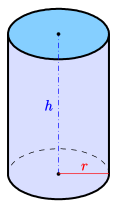
\includegraphics[keepaspectratio]{index_files/mediabag/files/lektionen_hs25/251027_funktionen/Zylinder.pdf}}

}

\caption{Zylinder}

\end{figure}%

Die Formel für die Berechnung des Volumens lautet

\[
v = \pi \cdot r^2 \cdot h
\]

Zerlegen Sie dazu die Berechnung in zwei Teile. Definieren Sie zuerst
eine Funkiton für die Berechnung der Bodenfläche und verwenden Sie diese
anschliessend in einer Funktion zur Berechnung des Volumens.

Für die Kreiszahl \(\pi\) können Sie das Modul \texttt{math}
importieren. Dies stellt Ihnen mit dem Befehl \texttt{math.pi} \(\pi\)
in einer grossen genauigkeit zur Verfügung.

\begin{Shaded}
\begin{Highlighting}[numbers=left,,]
\CommentTok{\# }\AlertTok{TODO}\CommentTok{: implementieren Sie hier Ihre Funktionen}
\end{Highlighting}
\end{Shaded}

\subsection{Berechnung der kinetischen Energie eines
Körpers}\label{berechnung-der-kinetischen-energie-eines-kuxf6rpers}

Die kinetische Energie eines Körpers berechnet sich nach der Formel

\[
E_{kin} = \frac{1}{2} \cdot m \cdot v^2
\]

wobei \(m\) für die Masse des Körpers und \(v\) für dessen
Geschwindigkeit steht. Implementieren Sie eine Funktion für die
Berechnung der kinetischen Energie eines Körpers. Beachten Sie dabei,
dass experimentell lediglich Daten über die Masse des Körpers, die
zurückgelegte Strecke des Körpers sowie die dafür erforderliche Zeit
zugänglich sind.

\begin{Shaded}
\begin{Highlighting}[numbers=left,,]
\CommentTok{\# }\AlertTok{TODO}\CommentTok{: implementieren Sie hier Ihre Funktionen}
\end{Highlighting}
\end{Shaded}

\section{Musterlösungen}\label{musterluxf6sungen-2}

\subsection{Berechnung des Volumnens eines
Zylinders}\label{berechnung-des-volumnens-eines-zylinders}

\begin{Shaded}
\begin{Highlighting}[numbers=left,,]
\ImportTok{import}\NormalTok{ math}

\KeywordTok{def}\NormalTok{ kreisflaeche(r : }\BuiltInTok{float}\NormalTok{) }\OperatorTok{{-}\textgreater{}} \BuiltInTok{float}\NormalTok{:}
\NormalTok{    area }\OperatorTok{=}\NormalTok{ math.pi }\OperatorTok{*}\NormalTok{ r }\OperatorTok{**} \DecValTok{2}
    \ControlFlowTok{return}\NormalTok{ area}

\KeywordTok{def}\NormalTok{ zylindervolumen(r : }\BuiltInTok{float}\NormalTok{, h : }\BuiltInTok{float}\NormalTok{) }\OperatorTok{{-}\textgreater{}} \BuiltInTok{float}\NormalTok{:}
\NormalTok{    bodenflaeche }\OperatorTok{=}\NormalTok{ kreisflaeche(r)}
\NormalTok{    volumen }\OperatorTok{=}\NormalTok{ bodenflaeche }\OperatorTok{*}\NormalTok{ h}
    \ControlFlowTok{return}\NormalTok{ volumen}
\end{Highlighting}
\end{Shaded}

\subsection{Berechnung der kinetischen Energie eines
Körpers}\label{berechnung-der-kinetischen-energie-eines-kuxf6rpers-1}

\begin{Shaded}
\begin{Highlighting}[numbers=left,,]
\KeywordTok{def}\NormalTok{ geschwindigkeit(s: }\BuiltInTok{float}\NormalTok{, t: }\BuiltInTok{float}\NormalTok{) }\OperatorTok{{-}\textgreater{}} \BuiltInTok{float}\NormalTok{:}
    \CommentTok{"""Berechnet die Geschwindigkeit v aus zurückgelegter Strecke und}
\CommentTok{    Zeit. }

\CommentTok{    Args:}
\CommentTok{        s: Die zurückgelegte Strecke (in Metern).}
\CommentTok{        t: Die dafür benötigte Zeit (in Sekunden).}

\CommentTok{    Returns:}
\CommentTok{        Die berechnete Geschwindigkeit v (in m/s).}
\CommentTok{    """}
\NormalTok{    v }\OperatorTok{=}\NormalTok{ s }\OperatorTok{/}\NormalTok{ t}
    \ControlFlowTok{return}\NormalTok{ v}


\KeywordTok{def}\NormalTok{ kinetische\_energie(m: }\BuiltInTok{float}\NormalTok{, s: }\BuiltInTok{float}\NormalTok{, t: }\BuiltInTok{float}\NormalTok{) }\OperatorTok{{-}\textgreater{}} \BuiltInTok{float}\NormalTok{:}
    \CommentTok{"""Berechnet die kinetische Energie eines Körpers basierend auf}
\CommentTok{    experimentellen Daten. }

\CommentTok{    Die Funktion berechnet zuerst die Geschwindigkeit v aus s und t}
\CommentTok{    mithilfe der Funktion \textquotesingle{}geschwindigkeit\textquotesingle{} und wendet dann die Formel}
\CommentTok{    E\_kin = 0.5 * m * v\^{}2 an.}

\CommentTok{    Args:}
\CommentTok{        m: Die Masse des Körpers (in Kilogramm).}
\CommentTok{        s: Die zurückgelegte Strecke (in Metern).}
\CommentTok{        t: Die dafür benötigte Zeit (in Sekunden).}

\CommentTok{    Returns:}
\CommentTok{        Die berechnete kinetische Energie E\_kin (in Joule).}
\CommentTok{    """}
\NormalTok{    v }\OperatorTok{=}\NormalTok{ geschwindigkeit(s, t)}
\NormalTok{    e\_kin }\OperatorTok{=}\NormalTok{ (m }\OperatorTok{*}\NormalTok{ v }\OperatorTok{**} \DecValTok{2}\NormalTok{) }\OperatorTok{/} \DecValTok{2}
    \ControlFlowTok{return}\NormalTok{ e\_kin}
\end{Highlighting}
\end{Shaded}

\chapter{Datenstrukturen: Listen}\label{datenstrukturen-listen}

\section{Daten in Listen speichern}\label{daten-in-listen-speichern}

Bisher hatten Sie Datentypen wie \texttt{int}, \texttt{float}
\texttt{str} und \texttt{bool} angeschaut. Wir möchten nun mehrere Werte
in einer Liste speichern.

Ich möchte zum Beispiel alle Wochentagekürzel in einer Liste speichern.
Um eine Liste im Code zu speichern, muss man die Liste mit \texttt{{[}}
beginnen und mit \texttt{{]}} enden. Die Elemente werden mit einem Komma
\texttt{,} getrennt.

\begin{Shaded}
\begin{Highlighting}[numbers=left,,]
\NormalTok{wochentage }\OperatorTok{=}\NormalTok{ [}\StringTok{"Mo"}\NormalTok{, }\StringTok{"Di"}\NormalTok{, }\StringTok{"Mi"}\NormalTok{, }\StringTok{"Do"}\NormalTok{, }\StringTok{"Fr"}\NormalTok{, }\StringTok{"Sa"}\NormalTok{, }\StringTok{"So"}\NormalTok{]}
\BuiltInTok{print}\NormalTok{(wochentage)}
\end{Highlighting}
\end{Shaded}

\subsection{Aufgabe: Monatsliste
erstellen}\label{aufgabe-monatsliste-erstellen}

Machen Sie eine Liste mit den 12 Monaten und printen Sie die Monate.

\begin{Shaded}
\begin{Highlighting}[numbers=left,,]
\CommentTok{"""Aufgabe: Monatsliste erstellen"""}

\NormalTok{monate }\OperatorTok{=} \CommentTok{\# }\AlertTok{TODO}
\BuiltInTok{print}\NormalTok{(monate)}
\end{Highlighting}
\end{Shaded}

\section{Index}\label{index}

Die Werte werden durchnummeriert. Die dazugehörige Nummer eines Werts
nennen wir den \emph{Index}.

Das erste Element hat den Index 0!

Um ein Element aus der Liste auszugeben können wir nach dem
Variablennamen die eckigen Klammen und den Index angeben.

\texttt{wochentage{[}0{]}} ist \texttt{"Mo"}. \texttt{wochentage{[}1{]}}
ist \texttt{"Di"}.

\subsection{Aufgabe: Index lesen}\label{aufgabe-index-lesen}

Lesen Sie den Codeblock und schrieben Sie hier auf, was Sie als Output
erwarten, \emph{bevor} Sie den Codeblock ausführen!

Ich erwarte, dass das Programm folgendes ausgibt:

\begin{verbatim}
TODO: Diese Zeile ersetzen.
\end{verbatim}

\begin{Shaded}
\begin{Highlighting}[numbers=left,,]
\NormalTok{lieblingstag }\OperatorTok{=}\NormalTok{ wochentage[}\DecValTok{3}\NormalTok{]}
\BuiltInTok{print}\NormalTok{(}\SpecialStringTok{f"Mein Lieblingstag ist }\SpecialCharTok{\{}\NormalTok{lieblingstag}\SpecialCharTok{\}}\SpecialStringTok{."}\NormalTok{)}
\end{Highlighting}
\end{Shaded}

\section{Überschreiben von
Elementen}\label{uxfcberschreiben-von-elementen}

Wir betrachten in diesem Kapitel eine Liste mit Zahlen (\texttt{int}).
Wir speichern für jeden Monat die Länge des Monats. Im Falle eines
Schaltjahrs möchten wir den Februar überschreiben mit 29. Studieren Sie
das Beispiel:

\begin{Shaded}
\begin{Highlighting}[numbers=left,,]
\NormalTok{monatslaenge }\OperatorTok{=}\NormalTok{ [}\DecValTok{31}\NormalTok{, }\DecValTok{28}\NormalTok{, }\DecValTok{31}\NormalTok{, }\DecValTok{30}\NormalTok{, }\DecValTok{31}\NormalTok{, }\DecValTok{30}\NormalTok{, }\DecValTok{31}\NormalTok{, }\DecValTok{31}\NormalTok{, }\DecValTok{30}\NormalTok{, }\DecValTok{31}\NormalTok{, }\DecValTok{30}\NormalTok{, }\DecValTok{31}\NormalTok{]}
\NormalTok{schaltjahr }\OperatorTok{=} \VariableTok{True}
\ControlFlowTok{if}\NormalTok{ schaltjahr:}
\NormalTok{    monatslaenge[}\DecValTok{1}\NormalTok{] }\OperatorTok{=} \DecValTok{29} \CommentTok{\# Der Februar hat den Index 2.}
\BuiltInTok{print}\NormalTok{(monatslaenge)}
\end{Highlighting}
\end{Shaded}

\section{Schleifen}\label{schleifen}

Listen eignen sich hervorragend um eine for-Schleife zu bauen.
Betrachten Sie das Beispiel, welches den Index als \texttt{i} und den
Wochentagsname als \texttt{wochentag} ausgibt. Die Liste
\texttt{wochentage} möchten wir auf keinen Fall überschreiben. Also
verwenden wir für die \emph{Laufvaribale} andere Variablennamen. In
diesem Fall nehmen wir \texttt{i} für den Index und \texttt{wochentag}
(Singular) für den Name des Tages.

\begin{Shaded}
\begin{Highlighting}[numbers=left,,]
\ControlFlowTok{for}\NormalTok{ i, wochentag }\KeywordTok{in} \BuiltInTok{enumerate}\NormalTok{(wochentage):}
    \BuiltInTok{print}\NormalTok{(}\SpecialStringTok{f"}\SpecialCharTok{\{}\NormalTok{i}\SpecialCharTok{\}}\SpecialStringTok{: }\SpecialCharTok{\{}\NormalTok{wochentag}\SpecialCharTok{\}}\SpecialStringTok{"}\NormalTok{)}
\end{Highlighting}
\end{Shaded}

Falls Sie den Index nicht benötigen, können Sie die Schleife mit
\texttt{for\ wochentag\ in\ wochentage:} machen.

\subsection{Aufgabe: Monatsschleife
komplettieren}\label{aufgabe-monatsschleife-komplettieren}

Erstellen Sie eine Schleife, welche folgendes Ausgibt:

\begin{verbatim}
Der Januar hat 31 Tage.
Der Februar hat 29 Tage.
Der März hat 31 Tage.
Der April hat 30 Tage.
Der Mai hat 31 Tage.
Der Juni hat 30 Tage.
Der Juli hat 31 Tage.
Der August hat 31 Tage.
Der September hat 30 Tage.
Der Oktober hat 31 Tage.
Der November hat 30 Tage.
Der Dezember hat 31 Tage.
\end{verbatim}

\begin{Shaded}
\begin{Highlighting}[numbers=left,,]
\CommentTok{"""Aufgabe: Monatsschleife komplettieren"""}

\ControlFlowTok{for}\NormalTok{ ... m\_name }\KeywordTok{in}\NormalTok{ ...:}
\NormalTok{    laenge }\OperatorTok{=}\NormalTok{ ... i ...}
    \BuiltInTok{print}\NormalTok{(}\SpecialStringTok{f"Der }\SpecialCharTok{\{}\NormalTok{m\_name}\SpecialCharTok{\}}\SpecialStringTok{ hat }\SpecialCharTok{\{}\NormalTok{laenge}\SpecialCharTok{\}}\SpecialStringTok{ Tage."}\NormalTok{)}
\end{Highlighting}
\end{Shaded}

\section{Länge}\label{luxe4nge}

Mit der Funktion \texttt{len(obj)} kann man die Länge der Liste
\texttt{obj} abfragen.

\begin{Shaded}
\begin{Highlighting}[numbers=left,,]
\CommentTok{"""Beispiel für len(obj)"""}
\BuiltInTok{print}\NormalTok{(}\SpecialStringTok{f"Die Woche hat }\SpecialCharTok{\{}\BuiltInTok{len}\NormalTok{(wochentage)}\SpecialCharTok{\}}\SpecialStringTok{ Tage."}\NormalTok{)}
\end{Highlighting}
\end{Shaded}

\section{Ergänzen und entfernen}\label{erguxe4nzen-und-entfernen}

Mit der Methode \texttt{append} kann ein Element am Ende der Liste
hinzufügen und mit \texttt{pop} wieder entfernen.

\begin{Shaded}
\begin{Highlighting}[numbers=left,,]
\NormalTok{tasks }\OperatorTok{=}\NormalTok{ [}\StringTok{"einkaufen"}\NormalTok{, }\StringTok{"spazieren gehen"}\NormalTok{, }\StringTok{"staubsaugen"}\NormalTok{]}
\NormalTok{tasks.append(}\StringTok{"essen"}\NormalTok{)}
\BuiltInTok{print}\NormalTok{(}\SpecialStringTok{f"Neu ist auch \textquotesingle{}essen\textquotesingle{} auf der Taskliste: }\SpecialCharTok{\{}\NormalTok{tasks}\SpecialCharTok{\}}\SpecialStringTok{"}\NormalTok{)}

\NormalTok{tasks.pop(}\DecValTok{1}\NormalTok{)}
\BuiltInTok{print}\NormalTok{(}\SpecialStringTok{f"Welcher Task ist nun erledigt? }\SpecialCharTok{\{}\NormalTok{tasks}\SpecialCharTok{\}}\SpecialStringTok{"}\NormalTok{)}

\NormalTok{tasks.pop()}
\BuiltInTok{print}\NormalTok{(}\StringTok{"Wird kein Index angegeben, so wird das letzte Element"}
      \SpecialStringTok{f"in der Liste entfernt: }\SpecialCharTok{\{}\NormalTok{tasks}\SpecialCharTok{\}}\SpecialStringTok{"}\NormalTok{)}
\end{Highlighting}
\end{Shaded}

\section{Aufgabe: Fibonacci}\label{aufgabe-fibonacci}

Die Fibonacci Reihe lautet 1, 1, 2, 3, 5, 8, 13, 8+13, \ldots{}

Die Summe der letzten zwei Zahlen ergeben die nächste Zahl.

Ergänzen Sie den Code, damit die Folge länger wird. Editieren Sie
Stellen mit drei Punkten.

\begin{Shaded}
\begin{Highlighting}[numbers=left,,]
\CommentTok{"""Aufgabe: Fibonacci"""}

\NormalTok{fibonacci: }\BuiltInTok{list} \OperatorTok{=}\NormalTok{ [}\DecValTok{1}\NormalTok{, }\DecValTok{1}\NormalTok{, }\DecValTok{2}\NormalTok{, }\DecValTok{3}\NormalTok{, }\DecValTok{5}\NormalTok{, }\DecValTok{8}\NormalTok{, }\DecValTok{13}\NormalTok{] }\CommentTok{\# Diese Zeile nicht verändern.}
\ControlFlowTok{for}\NormalTok{ \_ }\KeywordTok{in} \BuiltInTok{range}\NormalTok{(}\DecValTok{4}\NormalTok{):}
\NormalTok{    n }\OperatorTok{=}\NormalTok{ ... }\CommentTok{\# Die Länge von der Folge}
\NormalTok{    fibonacci ... (fibonacci ... }\OperatorTok{+}\NormalTok{ fibonacci ...)}
    \BuiltInTok{print}\NormalTok{(fibonacci)}
\end{Highlighting}
\end{Shaded}

\section{Aufgabe: zeichne Chomp}\label{aufgabe-zeichne-chomp}

Wie am Anfang der Lektion mündlich besprochen kodieren wir eine
Situation von \href{https://en.wikipedia.org/wiki/Chomp}{Chomp}.

\begin{figure}[H]

{\centering \pandocbounded{\includegraphics[keepaspectratio]{files/lektionen_hs25/251110_listen/Chomp_gameplay.png}}

}

\caption{Chomp\_gameplay}

\end{figure}%

Die dritte Situation beschreiben wir als Liste
\texttt{{[}4,\ 3,\ 3,\ 3,\ 2{]}}.

Schreiben Sie eine Funktion
\texttt{zeichne\_chomp(chomp:\ list)\ -\textgreater{}\ None} welche die
Situation zeichnet.

\begin{Shaded}
\begin{Highlighting}[numbers=left,,]
\CommentTok{"""Aufgabe: zeichne Chomp"""}
\ImportTok{from}\NormalTok{ pytamaro.de }\ImportTok{import} \OperatorTok{*}

\KeywordTok{def}\NormalTok{ zeichne\_chomp(chomp: }\BuiltInTok{list}\NormalTok{) }\OperatorTok{{-}\textgreater{}} \VariableTok{None}\NormalTok{:}
\NormalTok{    zelle }\OperatorTok{=}\NormalTok{ kombiniere(}
\NormalTok{        rechteck(}\DecValTok{68}\NormalTok{, }\DecValTok{38}\NormalTok{, rgb\_farbe(}\DecValTok{153}\NormalTok{, }\DecValTok{103}\NormalTok{, }\DecValTok{69}\NormalTok{)),}
\NormalTok{        rechteck(}\DecValTok{70}\NormalTok{, }\DecValTok{40}\NormalTok{, rgb\_farbe(}\DecValTok{51}\NormalTok{, }\DecValTok{34}\NormalTok{, }\DecValTok{23}\NormalTok{)),        }
\NormalTok{    )}
\NormalTok{    leere\_zelle }\OperatorTok{=}\NormalTok{ rechteck(}\DecValTok{70}\NormalTok{, }\DecValTok{40}\NormalTok{, weiss)}
\NormalTok{    tafel }\OperatorTok{=}\NormalTok{ leere\_grafik()}
\NormalTok{    maximum }\OperatorTok{=} \CommentTok{\# }\AlertTok{TODO}\CommentTok{ \# Groesse der erste Spalte}
    \ControlFlowTok{for}\NormalTok{ ... }\KeywordTok{in}\NormalTok{ chomp:}
\NormalTok{        spalte }\OperatorTok{=}\NormalTok{ leere\_grafik()}
\NormalTok{        ...}
\NormalTok{        ...}
\NormalTok{        tafel }\OperatorTok{=}\NormalTok{ neben(tafel, spalte)}
\NormalTok{    zeige\_grafik(tafel)}
\end{Highlighting}
\end{Shaded}

\begin{Shaded}
\begin{Highlighting}[numbers=left,,]
\CommentTok{\# Test für die Aufgabe}
\NormalTok{chomp\_test: }\BuiltInTok{list} \OperatorTok{=}\NormalTok{ [}\DecValTok{4}\NormalTok{, }\DecValTok{3}\NormalTok{, }\DecValTok{3}\NormalTok{, }\DecValTok{3}\NormalTok{, }\DecValTok{2}\NormalTok{]}
\NormalTok{zeichne\_chomp(chomp\_test)}
\end{Highlighting}
\end{Shaded}

\section{Aufgabe: spiele Chomp}\label{aufgabe-spiele-chomp}

Schreiben Sie eine Funktion
\texttt{chomp\_spielzug(chomp:\ list,\ spielzug:list)\ -\textgreater{}\ list}
welche aus der ersten Situation die neue Situation berechnet. Der
Spielzug ist eine Liste von der Form \texttt{{[}x,\ y{]}}.

Test:
\texttt{chomp\_spielzug({[}4,\ 3,\ 3,\ 3,\ 2{]},\ spielzug={[}3,\ 2{]})}
ergibt \texttt{{[}4,\ 3,\ 1,\ 1,\ 1{]}}

Bonusidee: Überprüfen Sie, ob der Spielzug überhaupt erlaubt ist.

\begin{Shaded}
\begin{Highlighting}[numbers=left,,]
\CommentTok{"""Aufgabe: programmiere den Spielzug in Chomp"""}

\CommentTok{\# }\AlertTok{TODO}\CommentTok{: Programmieren Sie es selber!}


\CommentTok{\# Hier können Sie den Code testen:}
\ControlFlowTok{assert}\NormalTok{ chomp\_spielzug([}\DecValTok{4}\NormalTok{, }\DecValTok{3}\NormalTok{, }\DecValTok{3}\NormalTok{, }\DecValTok{3}\NormalTok{, }\DecValTok{2}\NormalTok{], spielzug}\OperatorTok{=}\NormalTok{[}\DecValTok{3}\NormalTok{, }\DecValTok{2}\NormalTok{]) }\OperatorTok{==}\NormalTok{ [}\DecValTok{4}\NormalTok{, }\DecValTok{3}\NormalTok{, }\DecValTok{1}\NormalTok{, }\DecValTok{1}\NormalTok{, }\DecValTok{1}\NormalTok{]}
\end{Highlighting}
\end{Shaded}

\section{Übersicht}\label{uxfcbersicht}

Sie wissen, wie Sie

\begin{itemize}
\tightlist
\item
  eine Liste erstellen.
\item
  Elemente abfragen.
\item
  Elemente ändern.
\item
  mit einer Schleife durch die Liste gehen.
\item
  die Länge einer Liste bestimmen.
\item
  Elemente hinzufügen oder entfernen.
\end{itemize}

\section{Zusatzstoff}\label{zusatzstoff}

Weitere Infos und Features von Listen auf
\url{https://docs.python.org/3/library/stdtypes.html\#sequence-types-list-tuple-range}

Stichwörter: Slice, Spezialfall str, insert, in, join

\chapter{Datenstrukturen: Dictionary}\label{datenstrukturen-dictionary}

Dictionaries (Wörterbücher oder Maps) können mehrere Werte in einem
Objekt speichern, wie es Listen auch können. Die Werte haben aber keinen
Index sondern einen Schlüssel.

Ein \emph{Dictionary} in Python ist vergleichbar mit einem echten
Wörterbuch. Stellen Sie sich vor, Sie suchen die Telefonnummer (Wert)
einer Person (Schlüssel). In einem Python-Dictionary könnten Sie den
Namen der Person als Schlüssel und ihre Telefonnummer als Wert
speichern.

\begin{Shaded}
\begin{Highlighting}[numbers=left,,]
\CommentTok{"""Beispiel von einem dict"""}
\NormalTok{telefonbuch }\OperatorTok{=}\NormalTok{ \{}
    \StringTok{"Feuerwehr"}\NormalTok{: }\DecValTok{118}\NormalTok{,}
    \StringTok{"Polizei"}\NormalTok{: }\DecValTok{117}\NormalTok{,}
    \StringTok{"Ambulanz"}\NormalTok{: }\DecValTok{144}\NormalTok{,}
    \StringTok{"Rega"}\NormalTok{: }\DecValTok{1414}\NormalTok{,}
    \StringTok{"Beratung + Hilfe 147"}\NormalTok{: }\DecValTok{147}\NormalTok{,}
    \StringTok{"allgemeiner Notruf"}\NormalTok{: }\DecValTok{112}\NormalTok{,}
\NormalTok{\}}
\end{Highlighting}
\end{Shaded}

\section{Operationen für
Dictionaries}\label{operationen-fuxfcr-dictionaries}

\begin{itemize}
\item
  Erstellen eines Dictionaries: \texttt{dict\_name:\ dict\ =\ \{\}}

  Erstellt ein neues, leeres Dictionary mit dem Variablennamen
  \emph{dict\_name}.
\item
  Elemente aktualisieren:
  \texttt{dict\_name{[}\textquotesingle{}Schlüssel\textquotesingle{}{]}\ =\ \textquotesingle{}Neuer\ Wert\textquotesingle{}}

  Aktualisiert den Wert eines bestehenden Schlüssels oder fügt einen
  neuen Schlüssel mit dem angegebenen Wert hinzu, wenn er nicht
  existiert.
\item
  Elemente aufrufen:
  \texttt{var:\ str\ =\ dict\_name{[}\textquotesingle{}Schlüssel\textquotesingle{}{]}}

  \texttt{var} ist ein str mit dem Wert \texttt{’Neuer\ Wert’}. Man kann
  den Wert auch direkt zum printen oder anderes brauchen.
\item
  Elemente löschen:
  \texttt{dict\_name.pop(\textquotesingle{}Schlüssel\textquotesingle{})}

  Entfernt das Element mit dem angegebenen Schlüssel aus dem Dictionary.
\item
  Durch das Dictionary durchgehen:
  \texttt{for\ key,\ value\ in\ dict\_name.items()}

  Dieser Prozess heisst \emph{Iterieren}. Wir kennen ihn schon von der
  Liste oder Range. Iterieren heisst die Liste von Anfang bis Ende
  durchgehen. Jedes Mal wird in die Variablen \texttt{key},
  \texttt{vlaue} den Schlüssel, respektive den Wert des Eintrags
  zugewiesen. Sie können den Variablen auch andere Namen geben.
\end{itemize}

\subsection{Aufgabe: Vervollständigen Sie das
dict}\label{aufgabe-vervollstuxe4ndigen-sie-das-dict}

\begin{Shaded}
\begin{Highlighting}[numbers=left,,]
\CommentTok{"""Aufgabe: dict vervollständigen"""}

\NormalTok{voci }\OperatorTok{=}\NormalTok{ \{}
    \StringTok{"und"}\NormalTok{: }\StringTok{"and"}\NormalTok{,}
    \StringTok{"Auto"}\NormalTok{: ... ,}
    \StringTok{"Katze"}\NormalTok{: ... ,}
    \StringTok{"Tag"}\NormalTok{: ... ,}
    \StringTok{"Ende"}\NormalTok{: ... ,}
    \StringTok{"Familie"}\NormalTok{: ... ,}
    \StringTok{"Zuhause"}\NormalTok{: ... ,}
    \StringTok{"Name"}\NormalTok{: ... ,}
    \StringTok{"Menschen"}\NormalTok{: ... ,}
    \StringTok{"lesen"}\NormalTok{: ... ,}
    \StringTok{"Schule"}\NormalTok{: ... ,}
    \StringTok{"sprechen"}\NormalTok{: ... ,}
\NormalTok{\}}

\CommentTok{\# Test}
\BuiltInTok{print}\NormalTok{(voci[}\StringTok{"Schule"}\NormalTok{])}
\end{Highlighting}
\end{Shaded}

\subsection{Aufgabe: Schreiben Sie ein
dict}\label{aufgabe-schreiben-sie-ein-dict}

Schreiben Sie ein \texttt{dict} für Ihre Klasse, sodass der Nachname dem
Schlüssel/key und der Vorname dem Wert/value entspricht.

\begin{Shaded}
\begin{Highlighting}[numbers=left,,]
\CommentTok{"""Aufgabe: schreiben Sie ein dict"""}
\NormalTok{klasse }\OperatorTok{=}\NormalTok{ ...}
\end{Highlighting}
\end{Shaded}

\subsection{Aufgabe: Schleife}\label{aufgabe-schleife}

Iterieren Sie durch die ganze Liste, sodass alle aus der Klasse mit
\texttt{"Hallo\ {[}Vorname{]}\ {[}Nachname{]}"} begrüsst werden.

\begin{Shaded}
\begin{Highlighting}[numbers=left,,]
\CommentTok{"""Aufgabe: Schleife"""}
\ControlFlowTok{for}\NormalTok{ nachname, vorname }\KeywordTok{in}\NormalTok{ ... :}
    \BuiltInTok{print}\NormalTok{(}\SpecialStringTok{f"Hallo }\SpecialCharTok{\{}\NormalTok{vorname}\SpecialCharTok{\}}\SpecialStringTok{ }\SpecialCharTok{\{}\NormalTok{nachname}\SpecialCharTok{\}}\SpecialStringTok{"}\NormalTok{)}
\end{Highlighting}
\end{Shaded}

\subsection{Aufgabe: Selektion}\label{aufgabe-selektion}

Geben Sie nur die Nachnamen aus, welche ein \texttt{e} im Nachnamen
haben.

Tipp: Verwenden Sie
\texttt{if\ \textquotesingle{}e\textquotesingle{}\ in\ nachname:}

\begin{Shaded}
\begin{Highlighting}[numbers=left,,]
\CommentTok{"""Aufgabe: Selektion"""}

\NormalTok{...}
\end{Highlighting}
\end{Shaded}

\subsection{Aufgabe: Telefonliste}\label{aufgabe-telefonliste}

Erstellen Sie eine Liste \texttt{threedigtslist}, die nur die Namen der
Notfallorganisationen aus dem dict \texttt{telefonbuch} welche genau 3
Ziffern beinhalten.

\begin{Shaded}
\begin{Highlighting}[numbers=left,,]
\CommentTok{"""Aufgabe: Telefonliste"""}

\NormalTok{...}


\CommentTok{\# Test}
\ControlFlowTok{assert} \BuiltInTok{type}\NormalTok{(threedigtslist) }\OperatorTok{==} \BuiltInTok{list}
\ControlFlowTok{assert} \BuiltInTok{len}\NormalTok{(threedigtslist) }\OperatorTok{==} \DecValTok{5}
\ControlFlowTok{for}\NormalTok{ soultion }\KeywordTok{in}\NormalTok{ [}\StringTok{\textquotesingle{}Feuerwehr\textquotesingle{}}\NormalTok{, }\StringTok{\textquotesingle{}Polizei\textquotesingle{}}\NormalTok{, }\StringTok{\textquotesingle{}Ambulanz\textquotesingle{}}\NormalTok{, }\StringTok{\textquotesingle{}Beratung + Hilfe 147\textquotesingle{}}\NormalTok{, }\StringTok{\textquotesingle{}allgemeiner Notruf\textquotesingle{}}\NormalTok{]:}
    \ControlFlowTok{assert}\NormalTok{ soultion }\KeywordTok{in}\NormalTok{ threedigtslist}
\end{Highlighting}
\end{Shaded}

\chapter{Beurteilung von Algorithmen}\label{beurteilung-von-algorithmen}

Die Effizienz eines Algorithmus kann grundsätzlich nach seinem
Rechenaufwand oder Speicherbedarf beurteilt werden. Man spricht in
diesem Zusammenhang auch von Zeit- bzw. Platzkomplexität.

Wir haben uns mit dem Zählen von Vergleichen nur mit der Rechenaufwand,
also mit der Zeitkomplexität beschäftigt. Die Berechnungen werden sehr
stark vereinfacht.

\section{Bubblesort}\label{bubblesort}

Wenn wir mit dem Bubblesort \(n\) Objekte sortieren, haben wir \(n-1\)
Vergleiche im ersten Durchgang. Vereinfacht sagen wir einfach \(n\)
Vergleiche. Im schlimsten Fall, müssen ist das kleinste Element am
falschen Ende. Bei jedem Durchgang verschieben wir das Element nur um
einen Platz. Dass heisst wir müssen etwa \(n\) Durchgänge machen. Die
Laufzeit vom Bubblesort beträgt somit \(n \cdot n = n^2\).

\section{Mergesort}\label{mergesort}

\begin{figure}[H]

{\centering \pandocbounded{\includegraphics[keepaspectratio]{files/lektionen_hs25/251215_rekurisv/Mergesort_example.png}}

}

\caption{Mergesort\_example}

\end{figure}%

Bevor wir uns die Laufzeit von Mergesort anschauen, müssen wir
quantifizieren, wie oft wir die Listen aufteilen müssen. Haben wir 2
Elemente, separieren wir 1 Mal. Haben wir 4 Elemente separieren wir 2
mal.

\begin{longtable}[]{@{}ll@{}}
\toprule\noalign{}
len & Teilungen \\
\midrule\noalign{}
\endhead
\bottomrule\noalign{}
\endlastfoot
2 & 1 \\
4 & 2 \\
8 & 3 \\
16 & 4 \\
32 & 5 \\
64 & 6 \\
1024 & 10 \\
\end{longtable}

Diese Funktion, welche der Länge zur Anzahl Teilungen zuordnet, nennt
man \emph{Logarithmus zur Basis 2}. Man notiert sie wie folgt:
\(\log_2(n)\)

Auf jeder der \(\log_2(n)\) Ebene machen wir etwa \(n\) Vergleiche. Die
Laufzeit vom Mergesort beträgt somit \(n \cdot \log_2(n)\).

\chapter{Divide and Conquer}\label{divide-and-conquer}

Das Prinzip \emph{divide and conquer} (teile und herrsche) wurde am
Beispiel von Mergesort gezeigt, aber nicht explizit erwähnt. Dieses
Prinzip basiert auf der Idee, das kleine Probleme einfacher zu lösen
sind als grosse. Deshalb versucht man, das zu lösende Problem in
Teilprobleme aufzuteilen und diese, kleineren Probleme, zu lösen um
anschliessend die Teillösungen zu einer Lösung für das Ursprungsproblem
zusammenzusetzen.

Diese Idee wird oft durch \emph{Rekursion} umgesetzt. Der Begriff
Rekursion kann am besten am Beispiel einer Kindergeschichte erklärt
werden:

\begin{quote}
Es isch e mal en Maa gsi, de hät en hole Zah gha. I dem Zah häts es
Truckli gha und i däm Truckli häts es Briefli gha. I dem Briefli isch
gstande, es isch e mal en Maa gsi, de hät en hole Zah gha. I dem Zah
häts es Truckli gha und id däm Truckli häts es Briefli gha\ldots{}
\end{quote}

Rekursive Funktionen sind entsprechend Funktionen, die sich selber
aufrufen. Mergesort rief sich selber auf, um die Liste zu sortieren.

\section{Fibonacci-Folge}\label{fibonacci-folge}

Die
\href{https://de.wikipedia.org/wiki/Fibonacci-Folge}{Fibonacci-Folge} -
benannt nach dem Italienischen Mathematiker
\href{https://de.wikipedia.org/wiki/Leonardo_Fibonacci}{Leonardo
Fibonacci} - ist eine Zahlenfolge, in welcher die nächste Zahl die Summe
der beiden vorangegangenen Zahlen bildet. In Zahlen sieht das
folgendermassen aus:

\[
1, 1, 2, 3, 5, 8, 13, \dots
\]

Die Fibonacci-Folge wird rekursiv deifiniert:

\[
f_n = f_{n-1} + f_{n-2},\ \text{sofern}\ n \geq 3
\]

Sie haben die Fibonacci-Folge bei den Listen bereits programmiert.
Obwohl die Programmiung als Liste \emph{viel} effizienter ist, machen
wir hier eine Übung, Fibonacci als rekursive Funktion zu programmieren:

\begin{Shaded}
\begin{Highlighting}[numbers=left,,]
\CommentTok{"""Beispiel: fibonacci rekursiv definiert mit Printstatement"""}
\KeywordTok{def}\NormalTok{ fibonacci(n: }\BuiltInTok{int}\NormalTok{) }\OperatorTok{{-}\textgreater{}} \BuiltInTok{int}\NormalTok{:}
    \BuiltInTok{print}\NormalTok{(}\SpecialStringTok{f"Es wird fibonacci(}\SpecialCharTok{\{}\NormalTok{n}\SpecialCharTok{\}}\SpecialStringTok{) ausgeführt."}\NormalTok{)}
    \ControlFlowTok{if}\NormalTok{ n }\OperatorTok{\textless{}} \DecValTok{2}\NormalTok{:}
        \ControlFlowTok{return} \DecValTok{1}
    \ControlFlowTok{return}\NormalTok{ fibonacci(n}\OperatorTok{{-}}\DecValTok{1}\NormalTok{) }\OperatorTok{+}\NormalTok{ fibonacci(n}\OperatorTok{{-}}\DecValTok{2}\NormalTok{)}
\end{Highlighting}
\end{Shaded}

\subsection{Aufgabe: Fibonacci-Folge}\label{aufgabe-fibonacci-folge}

\begin{enumerate}
\def\labelenumi{\arabic{enumi}.}
\tightlist
\item
  Lesen Sie die Funktion \texttt{fibonacci}. Denken Sie im Kopf durch,
  was passiert, wenn Sie \texttt{fibonacci(0)} oder
  \texttt{fibonacci(1)} ausführen. Schreiben Sie Ihre Vermutung auf und
  führen Sie erst dann die Funktion aus. Vergleichen Sie Ihre Vermutung
  mit dem Resultat.
\item
  Denken Sie im Kopf durch, was passiert, wenn Sie \texttt{fibonacci(2)}
  ausführen. Schreiben Sie Ihre Vermutung auf und führen Sie erst dann
  die Funktion aus. Vergleichen Sie Ihre Vermutung mit dem Resultat.
\item
  Bonus: Denken Sie im Kopf durch, was passiert, wenn Sie
  \texttt{fibonacci(3)} ausführen. Schreiben Sie Ihre Vermutung auf und
  führen Sie erst dann die Funktion aus. Vergleichen Sie Ihre Vermutung
  mit dem Resultat.
\end{enumerate}

\section{Endlose Rekursion}\label{endlose-rekursion}

Wenn wir bei der Funktion \texttt{fibonacci} die Zeilen

\begin{Shaded}
\begin{Highlighting}[numbers=left,,]
    \ControlFlowTok{if}\NormalTok{ n }\OperatorTok{\textless{}} \DecValTok{2}\NormalTok{:}
        \ControlFlowTok{return} \DecValTok{1}
\end{Highlighting}
\end{Shaded}

weglassen würden, so würde die Funktion endlos sich selber aufrufen, wie
im Beispiel der Kindergeschichte.

Meistens wird dieses Problem mit Basisfälle gelöst.

\section{Beispiel: Anstossen}\label{beispiel-anstossen}

Gestern assen wir mit 6 Personen zu Abend. Vorgestern mit 140 Personen.
Wie oft schlagen die Gläser zusammen wenn alle miteinander anstossen?

Die Aufgabe können wir einfach reduzieren. Wenn ich die 6. Person am
Tisch bin, stosse ich mit 5 Personen an. Die 5 Personen müssen
untereinander noch anstossen. Das heisst \(a_n = a_{n-1} + (n-1)\).

Für die Rekursive Funktion, brauchen wir somit nur noch die Basisfälle.
In unserem Beispiel ist es: Wenn nur 0, 1 oder 2 Personen da sind, wie
oft wird angestossen?

\begin{longtable}[]{@{}ll@{}}
\toprule\noalign{}
Personen & Anstossen \\
\midrule\noalign{}
\endhead
\bottomrule\noalign{}
\endlastfoot
0 & 0 \\
1 & 0 \\
2 & 1 \\
\end{longtable}

\begin{Shaded}
\begin{Highlighting}[numbers=left,,]
\CommentTok{"""Aufgabe: finden Sie 2 Fehler"""}
\KeywordTok{def}\NormalTok{ anstossen(n: }\BuiltInTok{int}\NormalTok{) }\OperatorTok{{-}\textgreater{}} \BuiltInTok{int}\NormalTok{:}
    \CommentTok{\#\# Basisfälle}
    \ControlFlowTok{if}\NormalTok{ n }\OperatorTok{\textless{}=} \DecValTok{1}\NormalTok{:}
        \ControlFlowTok{return} \DecValTok{0}
    \ControlFlowTok{if}\NormalTok{ n }\OperatorTok{==} \DecValTok{2}\NormalTok{:}
        \ControlFlowTok{return} \DecValTok{2}

    \ControlFlowTok{return}\NormalTok{ anstossen(n}\OperatorTok{{-}}\DecValTok{1}\NormalTok{) }\OperatorTok{+}\NormalTok{ (n }\OperatorTok{+} \DecValTok{1}\NormalTok{)}
\end{Highlighting}
\end{Shaded}

\begin{Shaded}
\begin{Highlighting}[numbers=left,,]
\CommentTok{"""Test"""}
\ControlFlowTok{for}\NormalTok{ i }\KeywordTok{in} \BuiltInTok{range}\NormalTok{(}\DecValTok{10}\NormalTok{):}
    \BuiltInTok{print}\NormalTok{(}\SpecialStringTok{f"}\SpecialCharTok{\{}\NormalTok{i}\SpecialCharTok{\}}\SpecialStringTok{ Personen stossen }\SpecialCharTok{\{}\NormalTok{anstossen(i)}\SpecialCharTok{\}}\SpecialStringTok{ Mal an."}\NormalTok{)}

\NormalTok{i }\OperatorTok{=} \DecValTok{140}
\BuiltInTok{print}\NormalTok{(}\SpecialStringTok{f"}\SpecialCharTok{\{}\NormalTok{i}\SpecialCharTok{\}}\SpecialStringTok{ Personen stossen }\SpecialCharTok{\{}\NormalTok{anstossen(i)}\SpecialCharTok{\}}\SpecialStringTok{ Mal an."}\NormalTok{)}
\end{Highlighting}
\end{Shaded}

\subsection{Bonus: Die Gausssche
Summenformel}\label{bonus-die-gausssche-summenformel}

Der Deutsche Mathematiker Carl Friedich Gauss soll nach der Legende
seinen Mathematiklehrer bei einer Strafaufgabe überlistet haben. Gemäss
dieser Legende soll der Lehrer Gauss (und seinen Klassenkameraden) den
Auftrag gegen haben, die Zahlen von 1 bis 100 zusammenzuzählen.

Gauss soll nach kurzer Zeit mit der Lösung zum Lehrer gegangen sein.
Gauss' Lösung basierte auf folgender Formel:

\[
1 + 2 + 3 + ... + (n-1) + n = \sum_{k=1}^{n}k = \frac{n(n+1)}{2}
\]

Diese Formel kann direkt als Funktion implementiert werden. Das
entsprechende Beispiel finden sie in der folgenden Zelle.

\begin{Shaded}
\begin{Highlighting}[numbers=left,,]
\KeywordTok{def}\NormalTok{ gauss\_direct(n : }\BuiltInTok{int}\NormalTok{) }\OperatorTok{{-}\textgreater{}} \BuiltInTok{int}\NormalTok{:}
    \ControlFlowTok{return} \BuiltInTok{int}\NormalTok{((n}\OperatorTok{*}\NormalTok{(n}\OperatorTok{+}\DecValTok{1}\NormalTok{))}\OperatorTok{/}\DecValTok{2}\NormalTok{)}

\BuiltInTok{print}\NormalTok{(}\SpecialStringTok{f\textquotesingle{}Die Summe der Zahlen von 1 \textquotesingle{}}
      \SpecialStringTok{f\textquotesingle{}bis 100 ist }\SpecialCharTok{\{}\NormalTok{gauss\_direct(}\DecValTok{100}\NormalTok{)}\SpecialCharTok{\}}\SpecialStringTok{.\textquotesingle{}}\NormalTok{)}
\end{Highlighting}
\end{Shaded}

Alternativ kann die Formel aber auch rekursiv implementiert werden.
Entsprechend stellt sich die Frage, was wäre ein kleineres, aber
grundsätzlich gleichartiges Problem?\\
Im vorliegenden Fall wäre das einfachste gleichartige Problem, die Summe
aus einer Liste von Zahlen mit der Länge 1 und dem Wert 1 zu bilden.
Dann ist die Summe auch 1. Als Formel könnte man das so schreiben:

\[
\sum_{k=1}^{n}k = 1, \text{ sofern } n=1
\]

Daraus ergibt sich die Frage, wie man von \(n=100\) zu \(n=1\) kommt.

Für alle Fälle, in denen \(n>1\) ist, gilt

\[
\sum_{k=1}^{n}k = n + \sum_{k=1}^{n-1}k
\]

In dieser Formel kann nun immer wieder \(n-1\) eingesetzt werden. Das
ist die Rekursion.

Zusammengefasst kann dies folgendermassen dargestellt werden:

\[
\sum_{k=1}^{n}=
\left\{
    \begin{array}{lll}
        1,&n=1&\text{Basisfall}\\
        n+\sum\limits_{k=1}^{n-1}k,&\forall n > 1&\text{Rekursionsfall}
    \end{array}
\right.
\]

Der Basisfall ist einerseits der einfachste Fall und andererseits auch
der letzte Fall, der bearbeitet werden muss.\\
Beides ist wichtig. Dass der Basisfall der einfachste Fall ist, hilft
das Problem zu lösen. Dass der Basisfall der Lezte Fall ist, der
bearbeitet werden muss, ermöglicht es, die Rekursion zu beenden.

Im Rekursionsfall steht ``\(\forall n > 1\)''. Das \(\forall\) Zeichen
ist der sogenannte Allquantor und bedeutet hier ``\textbf{für alle}
\(n\) grösser als \(1\).

Das eine Problemlösung rekursiv implementiert wird, bedeutet, dass die
Funktion sich selber aufruft.\\
In der folgenden Zelle wird die gausssche Summenformel gemäss obiger
Darstellung rekursiv implementiert.

\begin{Shaded}
\begin{Highlighting}[numbers=left,,]
\CommentTok{"""Bonusaufgabe: Gauss Rekursiv"""}
\KeywordTok{def}\NormalTok{ gauss\_recursive(n : }\BuiltInTok{int}\NormalTok{) }\OperatorTok{{-}\textgreater{}} \BuiltInTok{int}\NormalTok{:}
    \CommentTok{\# }\AlertTok{TODO}\CommentTok{: rekursive Implementation des kleinen Gauss}
    \ControlFlowTok{pass}
    
\BuiltInTok{print}\NormalTok{(}\SpecialStringTok{f\textquotesingle{}Die Summe der Zahlen von 1 \textquotesingle{}}
      \SpecialStringTok{f\textquotesingle{}bis 100 ist }\SpecialCharTok{\{}\NormalTok{gauss\_recursive(}\DecValTok{100}\NormalTok{)}\SpecialCharTok{\}}\SpecialStringTok{.\textquotesingle{}}\NormalTok{)}
\end{Highlighting}
\end{Shaded}

\section{Fakultät}\label{fakultuxe4t-2}

Mit Fakultät (\(n!\)) wird in der Mathematik jene Funktion bezeichnet
mit der alle natürlichen Zahlen \(\leq n\) miteinander multipliziert
werden.

\[
n! = 1 \cdot 2 \cdot ... \cdot (n-1) \cdot n = \prod\limits_{k=1}^{n} k
\]

Als Besonderheit muss mann wissen, dass \(0! = 1\) gilt.

In Python kann dies mit einer \texttt{for} Schleife berechnet werden. In
der folgenden Zelle wird eine entsprechende Funktion definiert.

\begin{Shaded}
\begin{Highlighting}[numbers=left,,]
\KeywordTok{def}\NormalTok{ factorial\_loop(n : }\BuiltInTok{int}\NormalTok{) }\OperatorTok{{-}\textgreater{}} \BuiltInTok{int}\NormalTok{:}
    \CommentTok{"""result wird gleich 1 gesetzt, }
\CommentTok{    weil 1 das neutrale Element der}
\CommentTok{    Multiplikation ist """}
\NormalTok{    result }\OperatorTok{=} \DecValTok{1}
    \ControlFlowTok{for}\NormalTok{ i }\KeywordTok{in} \BuiltInTok{range}\NormalTok{(}\DecValTok{1}\NormalTok{, n}\OperatorTok{+}\DecValTok{1}\NormalTok{):}
\NormalTok{        result }\OperatorTok{*=}\NormalTok{ i}
    
    \ControlFlowTok{return}\NormalTok{ result}

\BuiltInTok{print}\NormalTok{(}\SpecialStringTok{f\textquotesingle{}Das Resultat von 5! ist \textquotesingle{}}
      \SpecialStringTok{f\textquotesingle{}}\SpecialCharTok{\{}\NormalTok{factorial\_loop(}\DecValTok{5}\NormalTok{)}\SpecialCharTok{\}}\SpecialStringTok{.\textquotesingle{}}\NormalTok{)}
\end{Highlighting}
\end{Shaded}

Die Funktion kann allerdings auch rekursiv definiert werden. Die
Definition sieht dann folgendermassen aus:

\[
n! =
\left\{
    \begin{array}{lll}
        1,&n=0 \lor n=1&\text{Basisfall}\\
        n \times (n - 1)!, &\forall n > 1& \text{Rekursionsfall}\\
    \end{array}
\right.
\]

Entsprechend kann eine Funktion zur Berechnung von \(n!\) auch rekursiv
implementiert werden.

\begin{Shaded}
\begin{Highlighting}[numbers=left,,]
\CommentTok{"""Aufgabe: Fakultät"""}
\KeywordTok{def}\NormalTok{ factorial\_recursive(n : }\BuiltInTok{int}\NormalTok{) }\OperatorTok{{-}\textgreater{}} \BuiltInTok{int}\NormalTok{:}
    \CommentTok{\# }\AlertTok{TODO}\CommentTok{: rekursive Implementation der Fakultätsfunktion}
    \ControlFlowTok{pass}
    
\BuiltInTok{print}\NormalTok{(}\SpecialStringTok{f\textquotesingle{}Das Resultat von 5! ist \textquotesingle{}}
      \SpecialStringTok{f\textquotesingle{}}\SpecialCharTok{\{}\NormalTok{factorial\_recursive(}\DecValTok{5}\NormalTok{)}\SpecialCharTok{\}}\SpecialStringTok{.\textquotesingle{}}\NormalTok{)}
\end{Highlighting}
\end{Shaded}

\section{Wörter umdrehen}\label{wuxf6rter-umdrehen}

Gesucht ist eine rekursive Funktion, welche ein Wort rückwärts schreibt
(bsp. Kantonsschule nach eluhcssnotnaK).

\begin{Shaded}
\begin{Highlighting}[numbers=left,,]
\CommentTok{"""Aufgabe: umdrehen"""}
\KeywordTok{def}\NormalTok{ reverse(s : }\BuiltInTok{str}\NormalTok{) }\OperatorTok{{-}\textgreater{}} \BuiltInTok{str}\NormalTok{:}
    \ControlFlowTok{if} \BuiltInTok{len}\NormalTok{(s) }\OperatorTok{==} \DecValTok{0} \KeywordTok{or} \BuiltInTok{len}\NormalTok{(s) }\OperatorTok{==} \DecValTok{1}\NormalTok{:}
        \ControlFlowTok{return}\NormalTok{ ...}
    \ControlFlowTok{else}\NormalTok{:}
\NormalTok{        head }\OperatorTok{=}\NormalTok{ s[}\DecValTok{0}\NormalTok{]}
\NormalTok{        tail }\OperatorTok{=}\NormalTok{ s[}\DecValTok{1}\NormalTok{:]}
        \ControlFlowTok{return}\NormalTok{ ...}
\end{Highlighting}
\end{Shaded}

\begin{Shaded}
\begin{Highlighting}[numbers=left,,]
\BuiltInTok{print}\NormalTok{(reverse(}\StringTok{\textquotesingle{}Kantonsschule\textquotesingle{}}\NormalTok{))}
\end{Highlighting}
\end{Shaded}

\section{Bonus: Anzahl Möglichkeiten zu
Zahlen}\label{bonus-anzahl-muxf6glichkeiten-zu-zahlen}

Ich Verkaufe eine Heft für 6 CHF. Wie viele Möglichkeiten gibt es 5 CHF
in Münzen (wir betrachten nur die Münzen 1, 2, 5 CHF).

\begin{itemize}
\tightlist
\item
  \(5+1\)
\item
  \(2+2+2\)
\item
  \(2+2+1+1\)
\item
  \(2+1+1+1+1\)
\end{itemize}

Es gibt 4 Möglichkeiten.

Um die Frage zu beantworten, kann man die Frage auch aufteilen. Die
grösste mögliche Münze ist 5. Also gibt es die Möglichkeiten mit einem 5
Fränkler zu bezahlen (1 Möglichkeit) oder ohne keinem 5 Fränkler zu
bezahlen (3 Möglichkeiten). Diese Anzahl Möglichkeiten zusammen addiert
ergibt die Möglichkeiten. Die Funktion benötigt 2 Argumente: Den zu
bezahlenden Betrag und die grösste erlaubte Münze.

\begin{Shaded}
\begin{Highlighting}[numbers=left,,]
\CommentTok{"""}
\CommentTok{Bonusaufgabe}
\CommentTok{Studieren Sie die Funktion und füllen Sie die Lücken mit den Auslassungspunkten.}
\CommentTok{"""}
\NormalTok{MUENZEN }\OperatorTok{=}\NormalTok{ [}\DecValTok{1000}\NormalTok{, }\DecValTok{200}\NormalTok{, }\DecValTok{100}\NormalTok{, }\DecValTok{50}\NormalTok{, }\DecValTok{20}\NormalTok{, }\DecValTok{10}\NormalTok{, }\DecValTok{5}\NormalTok{, }\DecValTok{2}\NormalTok{, }\DecValTok{1}\NormalTok{]}
\KeywordTok{def}\NormalTok{ anz\_zahlmöglichkeiten(}
\NormalTok{    value: }\BuiltInTok{int}\NormalTok{,}
\NormalTok{    largest\_index: }\BuiltInTok{int}\OperatorTok{=}\DecValTok{0}\NormalTok{,}
\NormalTok{    ) }\OperatorTok{{-}\textgreater{}} \BuiltInTok{int}\NormalTok{:}
    \CommentTok{"""Rekursive Funktion"""}
    \ControlFlowTok{if}\NormalTok{ value }\OperatorTok{\textless{}} \DecValTok{0}\NormalTok{:}
        \ControlFlowTok{return} \DecValTok{0}
    \ControlFlowTok{if}\NormalTok{ value }\OperatorTok{==} \DecValTok{0}\NormalTok{:}
        \ControlFlowTok{return} \DecValTok{1}
    \ControlFlowTok{if}\NormalTok{ largest\_index }\OperatorTok{+} \DecValTok{1} \OperatorTok{==} \BuiltInTok{len}\NormalTok{(MUENZEN):}
        \CommentTok{\# Pay with smales coins}
        \ControlFlowTok{return} \DecValTok{1}
    \CommentTok{\# Pay with largest Coin}
\NormalTok{    ret }\OperatorTok{=}\NormalTok{ ...}

    \CommentTok{\# Pay without larges coin}
\NormalTok{    ret }\OperatorTok{+=}\NormalTok{ ...}
    \ControlFlowTok{return}\NormalTok{ ret}

\BuiltInTok{print}\NormalTok{(anz\_zahlmöglichkeiten(}\DecValTok{5}\NormalTok{))}
\end{Highlighting}
\end{Shaded}

\begin{Shaded}
\begin{Highlighting}[numbers=left,,]
\BuiltInTok{print}\NormalTok{(anz\_zahlmöglichkeiten(}\DecValTok{500}\NormalTok{))  }\CommentTok{\# 6295434}
\CommentTok{\# print(anz\_zahlmöglichkeiten(700))  \# 40208370}
\CommentTok{\# print(anz\_zahlmöglichkeiten(1000)) \# 321335887}
\end{Highlighting}
\end{Shaded}

\begin{Shaded}
\begin{Highlighting}[numbers=left,,]
\CommentTok{"""}
\CommentTok{Bonusaufgabe}
\CommentTok{Printen Sie die Möglichkeiten!}

\CommentTok{[5]}
\CommentTok{[2, 2, 1]}
\CommentTok{[2, 1, 1, 1]}
\CommentTok{[1, 1, 1, 1, 1]}
\CommentTok{"""}
\NormalTok{MUENZEN }\OperatorTok{=}\NormalTok{ [}\DecValTok{1000}\NormalTok{, }\DecValTok{200}\NormalTok{, }\DecValTok{100}\NormalTok{, }\DecValTok{50}\NormalTok{, }\DecValTok{20}\NormalTok{, }\DecValTok{10}\NormalTok{, }\DecValTok{5}\NormalTok{, }\DecValTok{2}\NormalTok{, }\DecValTok{1}\NormalTok{]}
\KeywordTok{def}\NormalTok{ print\_zahlmöglichkeiten(...)}
\NormalTok{    ...}

\NormalTok{print\_zahlmöglichkeiten(}\DecValTok{5}\NormalTok{)}
\end{Highlighting}
\end{Shaded}

\chapter{Prüfungsvorbereitung 2}\label{pruxfcfungsvorbereitung-2}

\section{Lernziele}\label{lernziele}

Ich erwarte, dass Sie in der Lage sind

\begin{itemize}
\tightlist
\item
  eine Jupyter Arbeitsumgebung zu starten (auswendig);
\item
  Python Listen zu erstellen und zu verändern;
\item
  Werte aus Python Listen direkt oder mit Hilfe von \texttt{for}
  Schleifen zu verarbeiten;
\item
  Python Dictionaries zu erstellen und zu verändern;
\item
  Wert aus Python Dictionaries direkt oder mit Hilfe von \texttt{for}
  Schleifen zu verarbeiten sowie
\item
  rekursive Funktionen zu implementieren.
\end{itemize}

Die Inhalte der letzten Prüfung werden als Grundlagen vorausgesetzt. Die
Prüfung findet mit Papier und Bleistift statt. Als Hilfsmittel dürfen
Sie eine handschriftliche Zusammenfassung im Umfang einer Seite A4
mitbringen. Die Zusammenfassung darf alles ausser die Schritte zum Start
einer Jupyter Arbeitsumgebung enthalten.

\section{Listen}\label{listen}

\subsection{Listen erstellen}\label{listen-erstellen}

Das Fähnlein Fieselschweif besteht aus Donald Ducks Neffen Tick, Trick
und Track. Erstellen Sie eine Liste \texttt{fieselschweif} mit den drei
Mitgliedern.

\begin{Shaded}
\begin{Highlighting}[numbers=left,,]
\CommentTok{\# }\AlertTok{TODO}\CommentTok{: Liste erstellen}
\end{Highlighting}
\end{Shaded}

\subsection{Listen bearbeiten}\label{listen-bearbeiten}

Ergänzen Sie die vorher erstellte Liste `fieselschweif' um den Namen
\emph{Dagobert}.

\begin{Shaded}
\begin{Highlighting}[numbers=left,,]
\CommentTok{\# }\AlertTok{TODO}\CommentTok{: fieselschweif ergänzen}
\end{Highlighting}
\end{Shaded}

Dagobert gefällt es nicht im Fähnlein Fieselschweif. Entfernen Sie Ihn
wieder und lassen Sie Ihren Code den Text \emph{Dagobert hat das
Fähnlein Fieselschweif wieder verlassen.} ausgeben. Dagobert soll dabei
als Variabel \texttt{quitter} in den Code eingefügt werden.

\begin{Shaded}
\begin{Highlighting}[numbers=left,,]
\CommentTok{\# }\AlertTok{TODO}\CommentTok{: implementieren Sie die obige Vorgabe}
\end{Highlighting}
\end{Shaded}

\subsection{Über Listen iterieren}\label{uxfcber-listen-iterieren}

Gegeben sei eine Liste \texttt{numbers}. Die Liste beinhaltet die
natürlichen Zahlen von 1 bis 10
(\texttt{numbers\ =\ {[}1,\ 2,\ 3,\ 4,\ 5,\ 6,\ 7,\ 8,\ 9,\ 10{]}}).
Erstellen Sie mit Hilfe einer \texttt{for} schleife basierend auf der
Liste \texttt{numbers} eine neue Liste \texttt{triplet} welche aus den
Elementen der Dreierreihe des kleinen Einmaleins besteht.

\begin{Shaded}
\begin{Highlighting}[numbers=left,,]
\NormalTok{numbers }\OperatorTok{=}\NormalTok{ [}\DecValTok{1}\NormalTok{, }\DecValTok{2}\NormalTok{, }\DecValTok{3}\NormalTok{, }\DecValTok{4}\NormalTok{, }\DecValTok{5}\NormalTok{, }\DecValTok{6}\NormalTok{, }\DecValTok{7}\NormalTok{, }\DecValTok{8}\NormalTok{, }\DecValTok{9}\NormalTok{, }\DecValTok{10}\NormalTok{]}

\CommentTok{\# }\AlertTok{TODO}\CommentTok{: implementieren Sie die obige Vorgabe}
\end{Highlighting}
\end{Shaded}

\subsection{Python Dictionary
erstellen}\label{python-dictionary-erstellen}

Erstellen Sie ein Python Dictionary \texttt{mk}, welches die
Geschäftsadresse von Jacques Mock Schindler enthält. Die ersten zwei
Einträge erhalten Sie als Vorlage.

\begin{Shaded}
\begin{Highlighting}[numbers=left,,]
\NormalTok{mk }\OperatorTok{=}\NormalTok{ \{}
    \StringTok{\textquotesingle{}name\textquotesingle{}}\NormalTok{: }\StringTok{\textquotesingle{}Mock Schindler\textquotesingle{}}\NormalTok{,}
    \StringTok{\textquotesingle{}first\_name\textquotesingle{}}\NormalTok{: }\StringTok{\textquotesingle{}Jacques\textquotesingle{}}\NormalTok{,}
    \CommentTok{\# }\AlertTok{TODO}\CommentTok{: kompletieren Sie das Dictionary}
\NormalTok{\}}
\end{Highlighting}
\end{Shaded}

\subsection{Über ein Python Dictionary
iterieren}\label{uxfcber-ein-python-dictionary-iterieren}

Geben Sie den Inhalt des Dictionary \texttt{mk} mit Hilfe einer
\texttt{for} Schleife aus. Dabei soll die Ausgabe jedes Eintrags auf
einer neuen Zeile erfolgen.

\begin{Shaded}
\begin{Highlighting}[numbers=left,,]
\CommentTok{\# }\AlertTok{TODO}\CommentTok{: implementieren Sie obige Vorgabe}
\end{Highlighting}
\end{Shaded}

\subsection{Rekursion}\label{rekursion}

Ein Palindrom ist ein Wort, das in beide Richtungen gelesen werden kann.
Ein Beispiel für ein Palindrom ist \emph{Sugus}. Schreiben Sie eine
rekursive Funktion \texttt{palindrom\_tester}, welche testet, ob eine
gegebene Zeichenfolge ein Palindrom ist.

\emph{Hinweis}: Die einzelnen Zeichen eines Strings können wie die
Elemente einer Liste mit Hilfe eines Index abgerufen werden. Das erste
Zeichen eines Strings hat dabei den Index 0.

Damit Sie einfacher prüfen können, ob Ihre Funktion korrekt arbeitet,
übergeben Sie ihr ausschliesslich Strings in Kleinbuchstaben.

\begin{Shaded}
\begin{Highlighting}[numbers=left,,]
\CommentTok{\# }\AlertTok{TODO}\CommentTok{: implementieren Sie die obige Vorgabe}
\end{Highlighting}
\end{Shaded}

\section{Musterlösungen}\label{musterluxf6sungen-3}

\subsection{Listen erstellen}\label{listen-erstellen-1}

Das Fähnlein Fieselschweif besteht aus Donald Ducks Neffen Tick, Trick
und Track. Erstellen Sie eine Liste \texttt{fieselschweif} mit den drei
Mitgliedern.

\begin{Shaded}
\begin{Highlighting}[numbers=left,,]
\NormalTok{fieselschweif }\OperatorTok{=}\NormalTok{ [}\StringTok{\textquotesingle{}Tick\textquotesingle{}}\NormalTok{, }\StringTok{\textquotesingle{}Trick\textquotesingle{}}\NormalTok{, }\StringTok{\textquotesingle{}Track\textquotesingle{}}\NormalTok{]}
\end{Highlighting}
\end{Shaded}

\subsection{Listen bearbeiten}\label{listen-bearbeiten-1}

Ergänzen Sie die vorher erstellte Liste `fieselschweif' um den Namen
\emph{Dagobert}.

\begin{Shaded}
\begin{Highlighting}[numbers=left,,]
\NormalTok{fieselschweif.append(}\StringTok{\textquotesingle{}Dagobert\textquotesingle{}}\NormalTok{)}
\end{Highlighting}
\end{Shaded}

Dagobert gefällt es nicht im Fähnlein Fieselschweif. Entfernen Sie Ihn
wieder und lassen Sie Ihren Code den Text \emph{Dagobert hat das
Fähnlein Fieselschweif wieder verlassen.} ausgeben. Dagobert soll dabei
als Variabel \texttt{quitter} in den Code eingefügt werden.

\begin{Shaded}
\begin{Highlighting}[numbers=left,,]
\NormalTok{quitter }\OperatorTok{=}\NormalTok{ fieselschweif.pop()}
\BuiltInTok{print}\NormalTok{(}\SpecialStringTok{f\textquotesingle{}}\SpecialCharTok{\{}\NormalTok{quitter}\SpecialCharTok{\}}\SpecialStringTok{ hat das Fähnlein Fieslschweif wieder verlassen.\textquotesingle{}}\NormalTok{)}
\end{Highlighting}
\end{Shaded}

\subsection{Über Listen iterieren}\label{uxfcber-listen-iterieren-1}

Gegeben sei eine Liste \texttt{numbers}. Die Liste beinhaltet die
natürlichen Zahlen von 1 bis 10
(\texttt{numbers\ =\ {[}1,\ 2,\ 3,\ 4,\ 5,\ 6,\ 7,\ 8,\ 9,\ 10{]}}).
Erstellen Sie mit Hilfe einer \texttt{for} schleife basierend auf der
Liste \texttt{numbers} eine neue Liste \texttt{triplet} welche aus den
Elementen der Dreierreihe des kleinen Einmaleins besteht.

\begin{Shaded}
\begin{Highlighting}[numbers=left,,]
\NormalTok{numbers }\OperatorTok{=}\NormalTok{ [}\DecValTok{1}\NormalTok{, }\DecValTok{2}\NormalTok{, }\DecValTok{3}\NormalTok{, }\DecValTok{4}\NormalTok{, }\DecValTok{5}\NormalTok{, }\DecValTok{6}\NormalTok{, }\DecValTok{7}\NormalTok{, }\DecValTok{8}\NormalTok{, }\DecValTok{9}\NormalTok{, }\DecValTok{10}\NormalTok{]}

\NormalTok{triplet }\OperatorTok{=}\NormalTok{ []}

\ControlFlowTok{for}\NormalTok{ number }\KeywordTok{in}\NormalTok{ numbers:}
\NormalTok{    triplet.append(number }\OperatorTok{*} \DecValTok{3}\NormalTok{)}
\end{Highlighting}
\end{Shaded}

\subsection{Python Dictionary
erstellen}\label{python-dictionary-erstellen-1}

Erstellen Sie ein Python Dictionary \texttt{mk}, welches die
Geschäftsadresse von Jacques Mock Schindler enthält. Die ersten zwei
Einträge erhalten Sie als Vorlage.

\begin{Shaded}
\begin{Highlighting}[numbers=left,,]
\NormalTok{mk }\OperatorTok{=}\NormalTok{ \{}
    \StringTok{\textquotesingle{}name\textquotesingle{}}\NormalTok{: }\StringTok{\textquotesingle{}Mock Schindler\textquotesingle{}}\NormalTok{,}
    \StringTok{\textquotesingle{}first\_name\textquotesingle{}}\NormalTok{: }\StringTok{\textquotesingle{}Jacques\textquotesingle{}}\NormalTok{,}
    \StringTok{\textquotesingle{}street\textquotesingle{}}\NormalTok{: }\StringTok{\textquotesingle{}Rosenstrasse 1\textquotesingle{}}\NormalTok{,}
    \StringTok{\textquotesingle{}postcode\textquotesingle{}}\NormalTok{: }\DecValTok{8400}\NormalTok{,}
    \StringTok{\textquotesingle{}town\textquotesingle{}}\NormalTok{: }\StringTok{\textquotesingle{}Winterthur\textquotesingle{}}\NormalTok{,}
\NormalTok{\}}
\end{Highlighting}
\end{Shaded}

\subsection{Über ein Python Dictionary
iterieren}\label{uxfcber-ein-python-dictionary-iterieren-1}

Geben Sie den Inhalt des Dictionary \texttt{mk} mit Hilfe einer
\texttt{for} Schleife aus. Dabei soll die Ausgabe jedes Eintrags auf
einer neuen Zeile erfolgen.

\begin{Shaded}
\begin{Highlighting}[numbers=left,,]
\ControlFlowTok{for}\NormalTok{ key, value }\KeywordTok{in}\NormalTok{ mk.items():}
    \BuiltInTok{print}\NormalTok{(}\SpecialStringTok{f\textquotesingle{}}\SpecialCharTok{\{}\NormalTok{key}\SpecialCharTok{\}}\SpecialStringTok{: }\SpecialCharTok{\{}\NormalTok{value}\SpecialCharTok{\}}\SpecialStringTok{\textquotesingle{}}\NormalTok{)}
\end{Highlighting}
\end{Shaded}

\subsection{Rekursion}\label{rekursion-1}

Ein Palindrom ist ein Wort, das in beide Richtungen gelesen werden kann.
Ein Beispiel für ein Palindrom ist \emph{Sugus}. Schreiben Sie eine
rekursive Funktion \texttt{palindrom\_tester}, welche testet, ob eine
gegebene Zeichenfolge ein Palindrom ist.

\emph{Hinweis}: Die einzelnen Zeichen eines Strings können wie die
Elemente einer Liste mit Hilfe eines Index abgerufen werden. Das erste
Zeichen eines Strings hat dabei den Index 0.

Damit Sie einfacher prüfen können, ob Ihre Funktion korrekt arbeitet,
übergeben Sie ihr ausschliesslich Strings in Kleinbuchstaben.

\begin{Shaded}
\begin{Highlighting}[numbers=left,,]
\KeywordTok{def}\NormalTok{ palindrom\_tester(text):}
    \CommentTok{"""}
\CommentTok{    Prüft rekursiv, ob ein String ein Palindrom ist }
\CommentTok{    (vorwärts und rückwärts gelesen gleich).}
\CommentTok{    Beispiele: "Lagerregal", "Anna", "Reittier"}
\CommentTok{    """}
    \CommentTok{\# Vorverarbeitung: Kleinbuchstaben für einfacheren Vergleich}
    \CommentTok{\# (für den Fall, dass Sie sich nicht an den Tipp gehalten haben)}
\NormalTok{    text }\OperatorTok{=}\NormalTok{ text.lower()}
    
    \CommentTok{\# Rekursionsanker 1: Leerer String oder Einzelbuchstabe}
    \CommentTok{\# ist immer ein Palindrom.}
    \ControlFlowTok{if} \BuiltInTok{len}\NormalTok{(text) }\OperatorTok{\textless{}=} \DecValTok{1}\NormalTok{:}
        \ControlFlowTok{return} \VariableTok{True}
    
    \CommentTok{\# Rekursionsanker 2: Wenn erster und letzter Buchstabe }
    \CommentTok{\# nicht übereinstimmen,}
    \CommentTok{\# kann es kein Palindrom sein. Abbruch mit False.}
    \ControlFlowTok{if}\NormalTok{ text[}\DecValTok{0}\NormalTok{] }\OperatorTok{!=}\NormalTok{ text[}\OperatorTok{{-}}\DecValTok{1}\NormalTok{]:}
        \ControlFlowTok{return} \VariableTok{False}
    
    \CommentTok{\# Rekursionsschritt:}
    \CommentTok{\# Wenn die Ränder passen, prüfe den Teilstring ohne den}
    \CommentTok{\# ersten und letzten Buchstaben.}
    \ControlFlowTok{return}\NormalTok{ palindrom\_tester(text[}\DecValTok{1}\NormalTok{:}\OperatorTok{{-}}\DecValTok{1}\NormalTok{])}
\end{Highlighting}
\end{Shaded}





\end{document}
